\documentclass[12pt,a4paper]{report}
\usepackage{vntex} % Tiếng Việt
\usepackage{graphicx} % Chèn hình ảnh
\usepackage{fancyhdr} % Gói hỗ trợ tạo header và footer fancy
\usepackage{changepage} % Thay đổi lề

% Chèn code
\usepackage{listings} % Thêm gói listings để chèn code
\usepackage{xcolor} % Màu cho code
\lstset{
    language=Matlab,
    basicstyle=\footnotesize\ttfamily,
    numbers=none,
    numberstyle=\tiny\color{gray},
    stepnumber=1,
    numbersep=0.01pt,
    tabsize=2,
    breaklines=true,
    breakatwhitespace=false,
    xleftmargin=0cm, % for line numbers
    framexleftmargin=0cm, % for code frame
    keywordstyle=\color{blue},
    commentstyle=\color{green},
    stringstyle=\color{orange},
    frame=single,
    rulecolor=\color{black},
    basicstyle=\ttfamily,
}

% Footnote and References
\usepackage[style=numeric,backend=biber]{biblatex} % Sử dụng gói biblatex
\usepackage{capt-of} %  Footnote trong caption
\usepackage[perpage]{footmisc} % Đánh số lại chú thích mỗi trang

% Thiết lập bảng
\usepackage{array} % Gói hỗ trợ các bảng phức tạp
\usepackage{tabularx}
\usepackage{longtable} % Tạo bảng qua nhiều trang
\usepackage{cellspace}
\usepackage{diagbox} % Gói hỗ trợ tạo các ô chéo trong bảng
\usepackage{multirow}
\usepackage{makecell}
\usepackage{adjustbox}

% Thiết lập công thức toán học
\usepackage{amsmath} % Gói hỗ trợ các công thức toán học
\usepackage{amsfonts} % Gói hỗ trợ các ký hiệu toán học
\usepackage{amssymb} % Gói hỗ trợ các ký hiệu toán học
\usepackage{graphicx} % Gói hỗ trợ chèn hình ảnh
\usepackage{bm} % Chữ in đậm trong công thức toán 

% Thiết lập khác
\usepackage{tikz}
\usepackage{color}
\usepackage{subcaption}
\usepackage{framed}
\usepackage{float} % Để chèn hình ảnh vào đúng vị trí
\usepackage{fancyvrb} % Đưa dữ liệu dạng nguyên thủy vào

% Thiết lập kích thước
\usepackage{geometry}
\geometry{
    left=3cm,
    right=2cm,
    top=2.5cm,
    bottom=2.5cm,
}
\usepackage{hyperref} %Chèn link
\hypersetup{urlcolor=black,linkcolor=black,citecolor=black,colorlinks=true} % Màu cho các đường nét
\everymath{\color{black}}
\setlength{\headheight}{20pt}
\pagestyle{fancy}


\addbibresource{references.bib} 

%Header
\fancyhead{} % clear all header fields
\fancyhead[L]{
 \begin{tabular}{rl}
    \begin{picture}(25,15)(0,0)
    \put(0,-8){
\includegraphics[width=12mm, height=12mm]{pictures/hcmut.png}}
    %\put(0,-8){\epsfig{width=10mm,figure=hcmut.eps}}
   \end{picture}&
	%
\includegraphics[width=8mm, height=8mm]{hcmut.png} & %
	\begin{tabular}{l}
		\textbf{\bf \ttfamily Trường Đại Học Bách Khoa - ĐHQG TP.Hồ Chí Minh}\\
		\textbf{\bf \ttfamily Khoa Cơ Khí}\\
	\end{tabular} 	
 \end{tabular}
}
\fancyhead[R]{
	{\tiny \bf \quad} % Khoảng trắng nhỏ trong header bên phải
}

%Footer
\fancyfoot{} % clear all footer fields
\fancyfoot[L]{\scriptsize \ttfamily Đồ án Hệ thống truyền động}
\fancyfoot[R]{\scriptsize \ttfamily Trang {\thepage}/70}
\renewcommand{\headrulewidth}{0.3pt}
\renewcommand{\footrulewidth}{0.3pt}

\begin{document}
    \begin{titlepage}   
    \begin{center}
        \vspace*{-2cm} 
        \large
        \textbf{ĐẠI HỌC QUỐC GIA THÀNH PHỐ HỒ CHÍ MINH \\
        TRƯỜNG ĐẠI HỌC BÁCH KHOA\\
        KHOA CƠ KHÍ\\}
        \vspace{0.5cm}
        
\includegraphics[width=70mm, height=70mm]{pictures/hcmut.png} \\
        \rule{\linewidth}{0.5mm}\\
        \vspace{1cm}
        \LARGE
        \textbf{ĐỒ ÁN}\\                                                                                                                                                                                                                    
        \vspace*{0.5cm}
        \Huge
        \textbf{HỆ THỐNG TRUYỀN ĐỘNG}\\                                                                                                                                                                                                                                                                                                                                                                                                                                             
        \vspace{0.5cm}
        \rule{\linewidth}{0.5mm}\\
        \vspace{0.8cm}
        \vspace{1cm}
        \large
        GVHD: TS. PHẠM MINH TUẤN\\[0.5cm]
    \end{center}
        
    \vfill
    \large
    \begin{center}
        TP.HCM, \today
    \end{center}
\end{titlepage}
    \tableofcontents  
    \listoftables
    \listoffigures
    \newpage
    \Huge 
    \begin{center}
        \textbf{ĐỀ BÀI}
    \end{center}
    \normalsize
        \begin{figure}[H]
            \centering
            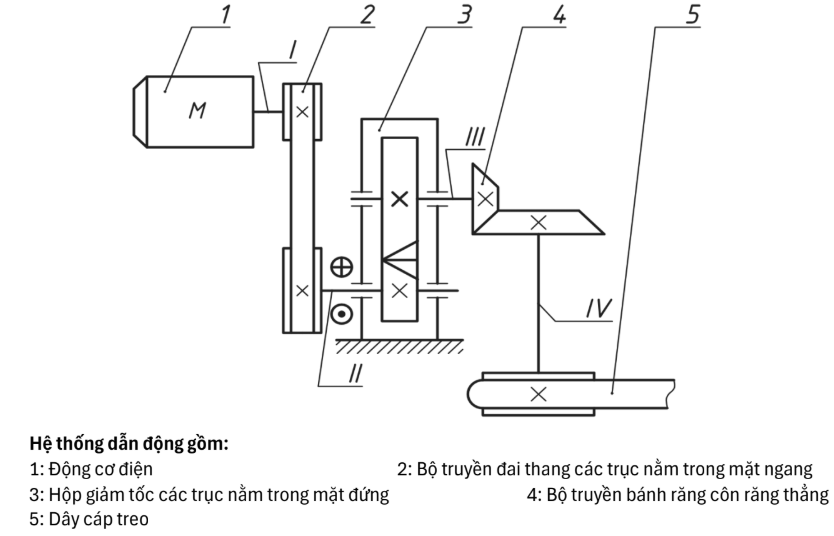
\includegraphics[width=1\textwidth]{pictures/topic.png}
        \end{figure}
        \begin{center}
            \begin{tabular}{|>{\centering\arraybackslash}m{8cm}|>{\centering\arraybackslash}m{5cm}|}
                \hline
                \textbf{Phương án} & \textbf{2}  \\
                \hline
                Công suất trục cáp, P (kW) & 2.5 \\
                \hline
                Số vòng quay trục cáp, n (vòng/phút) & 12 \\
                \hline
                Thời gian phục vụ, L (năm) & 5 \\
                \hline 
            \end{tabular}\\
            Quay một chiều, làm việc hai ca (1 năm làm việc 300 ngày, 1 ca làm việc 8 giờ)
        \end{center}
        \section*{LỜI MỞ ĐẦU}

    \hspace*{0.6cm}Trong cuộc sống hàng ngày, chúng ta có thể bắt gặp hệ thống truyền động khắp nơi. Có thể khẳng định rằng hệ thống truyền động đóng vai trò quan trọng trong các lĩnh vực công nghiệp cũng như đời sống con người. Đồ án thiết kế hệ thống truyền động là môn học cơ bản của ngành cơ khí, là môn có thể giúp sinh viên có cái nhìn cụ thể, thực tế hơn với các kiến thức và là cơ sở quan trọng để học các môn học khác sau này. Học tốt môn học này sẽ giúp cho sinh viên có thể tưởng tượng ra được công việc tương lai, qua đó có cách nhìn đúng đắn hơn về con đường học tập đồng thời tăng thêm lòng nhiệt huyết, yêu nghề cho mỗi sinh viên.

    Hệ thống truyền động con lăn là một trong những hệ thống cơ khí được ứng dụng rộng rãi trong nhiều lĩnh vực công nghiệp khác nhau như vận chuyển hàng hóa, dây chuyền sản xuất, hệ thống phân loại và các ứng dụng tự động hóa. Dù được ứng dụng trong trường hợp nào thì hệ thống truyền động con lăn cũng đều có chung nguyên lí hoạt động. Chuyển động quay của con lăn được truyền động từ động cơ thông qua một hộp giảm tốc rồi qua một bộ truyền khác như đai hoặc xích, giúp vận chuyển vật liệu một cách hiệu quả và tin cậy.

    Đồ án hệ thống truyền động là môn học giúp sinh viên khoa Cơ khí có bước đi chập chững, làm quen với công việc thiết kế mà mỗi người kỹ sư cơ khí sẽ gắn cuộc đời mình vào đó. Nó sẽ là giúp nâng cao những kĩ năng mà sinh viên đã được học từ những năm trước như về cơ khí, kĩ năng sử dụng phần mềm: Autocad, Autocad Mechanical, Autodesk Inventor\ldots cùng với những kiến thức trong những môn học nền tảng: Nguyên lí máy, Chi tiết máy, Dung sai và Kĩ thuật đo\ldots

    Trong quá trình thực hiện đồ án này, bọn em đã nhận được sự chỉ dẫn rất tận tình từ thầy \textbf{Phạm Minh Tuấn}, các thầy cô khác cũng như bạn bè trong ngành. Sự giúp đỡ của thầy cô và các bạn là nguồn động lực to lớn cổ vũ tinh thần cho bọn em để hoàn thành đồ án này và cả trong quá trình học tập, rèn luyện sau này. Do đây là lần đầu mà em thực hiện thiết kế và tính toán nên chắc chắn sẽ mắc phải những thiếu xót, sai lầm. Em rất mong nhận được sự góp ý chân thành từ phía quý thầy cô và các bạn. \\[1cm]
\hspace*{10cm}Sinh viên thực hiện \\[0.5cm]
\hspace*{8.5cm}Võ Hữu Dư - Võ Trần Trọng Khang\\
        \chapter{CHỌN ĐỘNG CƠ ĐIỆN VÀ PHÂN BỐ TỈ SỐ TRUYỀN}
    \section{CHỌN ĐỘNG CƠ ĐIỆN}
        \subsection{Hiệu suất chung của hệ thống}
            \begin{figure}[H]
                \centering
                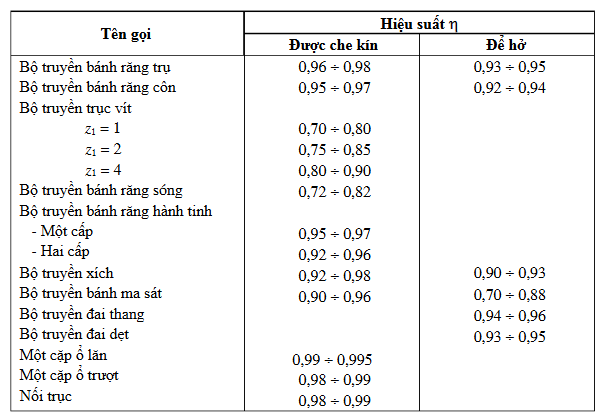
\includegraphics[width=0.8\textwidth]{pictures/table_1.png}
                \caption{Hiệu suất các bộ truyền chủ yếu}
            \end{figure}
            \hspace*{0.6cm}Dựa vào bảng hiệu suất các bộ truyền chủ yếu như trên, ta có:
            \begin{itemize}
                \item Hiệu suất của bộ truyền đai: $\eta_{d} = 0.94$.
                \item Hiệu suất của bộ truyền bánh răng trụ răng nghiêng để kín: $\eta_{br1} = 0.96$.
                \item Hiệu suất của bộ truyền bánh răng côn để hở: $\eta_{br2} = 0.92$.
                \item Hiệu suất của 2 cặp ổ lăn: $\eta_{ol}^2 = 0.99^2$.
            \end{itemize}
            \begin{center}
                $\eta_{ch}=\eta_{d} \cdot \eta_{br1} \cdot \eta_{br2} \cdot \eta_{ol}^2 = 0.94 \cdot 0.96 \cdot 0.92 \cdot 0.99^2 = 0.814 $.
            \end{center}
        \subsection{Công suất động cơ cần thiết}
            \begin{figure}[H]
                \centering
                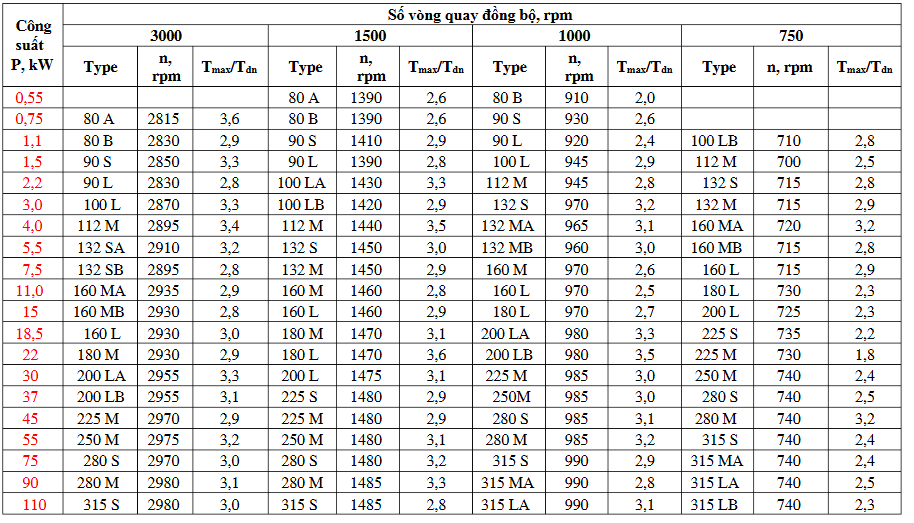
\includegraphics[width=1\textwidth]{pictures/table_2.png}
                \caption{Bảng chọn động cơ 3 pha không đồng bộ}
            \end{figure}
            \begin{center}
                $P_{dc}=\frac{P_{ct}}{\eta_{ch}} = \frac{2.5}{0.814} = 3.07 (kW)$.
            \end{center}
        \subsection{Xác định số vòng quay sơ bộ}
            \begin{figure}[H]
                \centering
                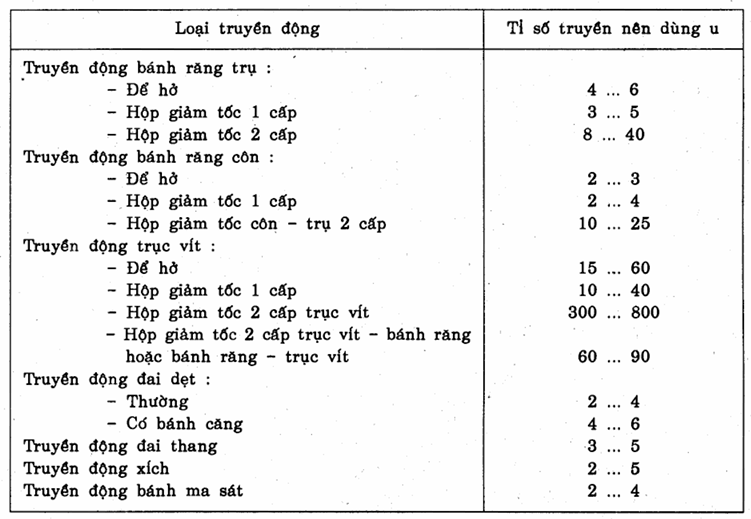
\includegraphics[width=0.8\textwidth]{pictures/table_3.png}
                \caption{Bảng chọn tỉ số truyền}
            \end{figure}
            \begin{itemize}
                \item Chọn tỉ số truyền \footnote{Tra bảng [2.4], tài liệu tham khảo \cite{tltk1} }: $u_{br1} = 5; u_{br2} = 6; u_{d} = 2$\\
                \item Tỷ số truyền hệ thống: $u_{ch}=u_{br1} \cdot u_{br2} \cdot u_{d}=\frac{n_{dc}}{n_{ct}} = 6 \cdot 5 \cdot 2 = 60$.\\
                \item Số vòng quay sơ bộ của động cơ: $n_{sb} = n_{ct} \cdot u_{ch} = 12 \cdot 60 = 720.$
            \end{itemize}
        \subsection{Chọn động cơ}
            \hspace*{0.6cm}Dựa vào bảng chọn Động cơ 3 pha Không đồng bộ, chọn lấy động cơ có công suất lớn hơn 3.07(kW) và gần nhất. Từ đó, ta có động cơ công suất 4(kW).\\
            \begin{table}[H]
                \centering
                \begin{tabular}{|>{\centering\arraybackslash}m{1.8cm}|>{\centering\arraybackslash}m{2.5cm}|>{\centering\arraybackslash}m{2.5cm}|>{\centering\arraybackslash}m{2.5cm}|>{\centering\arraybackslash}m{2.5cm}|>{\centering\arraybackslash}m{2.5cm}|}
                    \hline
                    \textbf{Động cơ} & \textbf{Số vòng quay động cơ $n_{dc}$ (vg/ph)} & \textbf{Tỷ số truyền chung $u_{ch}$} & \textbf{Bộ truyền đai thang} & \textbf{Bộ truyền bánh răng trụ kín $u_{br1}$} & \textbf{Bộ truyền bánh răng côn hở $u_{br2}$} \\ 
                    \hline
                    ĐC1 & 2895 & 241.25 & 2 & 12.5 & 9.65 \\
                    \hline
                    ĐC2 & 1440 & 120 & 2 & 11.2 & 5.36 \\
                    \hline
                    ĐC3 & 965 & 80.42 & 2 & 8 & 5.03 \\ 
                    \hline
                    ĐC4 & 720 & 60 & 1.5 & 8 & 5 \\
                    \hline 
                \end{tabular}
                \caption{Động cơ và phân phối tỉ số truyền}
                \label{tab:gear_ratios}
            \end{table}
            \hspace*{0.6cm}Chọn động cơ sao cho thỏa mản $P_{dc} > =P{ct}$ và $n_{dc} \approx n_{sb}$, ta chọn động cơ 4 (Động cơ 160MA).\\
            \hspace*{1.2cm}Động cơ 4: $P_{dc} = 4.0(kW); n_{dc} = 720(vg/ph); u_{ch} = 60; u_{br1} = 8; u_{br2} = 5; u_{d} = 1.5$.
    \section{PHÂN PHỐI TỈ SỐ TRUYỀN}
        \subsection{Công suất trên từng trục}
            \begin{itemize}
                \item $P_{III} = \frac{P_{ct}}{\eta_{br2}} = \frac{2.5}{0.92} = 2.72(kW)$.
                \item $P_{II} = \frac{P_{III}}{\eta_{br1}.\eta{ol}} = \frac{2.72}{0.96.0.99} = 2.86(kW)$.
                \item $P_{I} = \frac{P_{II}}{\eta_{d}.\eta{ol}} = \frac{2.86}{0.94.0.99} = 3.07(kW)$.
            \end{itemize}
        \subsection{Số vòng quay trên từng trục}
            \begin{itemize}
                \item $n_{II} = \frac{n_{dc}}{u_{d}} = \frac{720}{2} = 360$ (vg/ph). 
                \item $n_{III} = \frac{n_{II}}{u_{br1}} = \frac{360}{5} = 72$ (vg/ph).
                \item $n_{IV} = \frac{n_{III}}{u_{br2}} = \frac{72}{6} = $ (vg/ph).
            \end{itemize}
        \subsection{Moment xoắn trên trục}
            \begin{itemize}
                \item $T_{I} = 9.55.10^3.\frac{P_{I}}{n_{I}} = 9.55.10^3.\frac{3.07}{720} = 40.72(N.m).$
                \item $T_{II} = 9.55.10^3.\frac{P_{II}}{n_{II}} = 9.55.10^3.\frac{2.86}{360} = 75.87(N.m).$
                \item $T_{III} = 9.55.10^3.\frac{P_{III}}{n_{III}} = 9.55.10^3.\frac{2.72}{72} = 360.78(N.m).$
                \item $T_{IV} = 9.55.10^3.\frac{P_{IV}}{n_{IV}} = 9.55.10^3.\frac{2.5}{12} = 1989.58(N.m).$
            \end{itemize}
            \begin{table}[H]
                \centering
                \begin{tabular}{|>{\centering\arraybackslash}m{4.2cm}|>{\centering\arraybackslash}m{2.5cm}|>{\centering\arraybackslash}m{2.5cm}|>{\centering\arraybackslash}m{2.5cm}|>{\centering\arraybackslash}m{2.5cm}|}
                    \hline
                    \diagbox{\textbf{Thông số}}{\textbf{Trục}} & \textbf{I} & \textbf{II} & \textbf{III} & \textbf{IV} \\ 
                    \hline
                    Công suất (kW) & 3.07 & 2.86 & 2.72 & 2.5 \\
                    \hline
                    Tỷ số truyền & \multicolumn{1}{c|}{2} & \multicolumn{2}{c|}{5} & \multicolumn{1}{c|}{6}\\
                    \hline
                    Momen xoắn (N.m) & 40.72 & 75.87 & 360.78 & 1989.58 \\ 
                    \hline
                    Số vòng quay (vòng/ph) & 720 & 360 & 72 & 12 \\
                    \hline 
                \end{tabular}
                \caption{Đặc tính kỹ thuật hệ thống truyền động}
                \label{tab:technical_specifications}
            \end{table}
        \chapter{THIẾT KẾ BỘ TRUYỀN ĐAI THANG}
    \section*{2.0. THÔNG SỐ KỸ THUẬT BỘ TRUYỀN ĐAI THANG}
        \begin{itemize}
            \item Công suất trục động cơ: $P_{I} = 3.07(kW)$.
            \item Tỉ số truyền bộ truyền: $u_{d} = 2$.
            \item Số vòng quay bánh dẫn: $n_{I} = 720(rpm)$.
            \item Momen xoắn: $T_{I} = 40.72(N.m)$. 
        \end{itemize}
    \section{CHỌN LOẠI ĐAI VÀ TIẾT DIỆN}
        \hspace*{0.6cm}Kích thước bánh đai thang thường được chia làm 7 loại chính Z, A, B, C, D, E. Với bảng chọn dạng đai phụ thuộc vào công suất truyền của trục và vận tóc góc trục được thiết kế.\\
        \hspace*{0.6cm}Dựa vào bảng 4.3 tài liệu tham khảo \cite{gtctm}, với công suất trục động cơ $P_{I} = 3.07(kW)$ và số vòng quay bánh dẫn $n_{I} = 720(rpm)$, ta chọn được loại đai thang:\\  
        \begin{figure}[H]
            \centering
            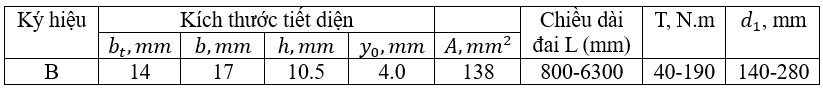
\includegraphics[width=1\textwidth]{pictures/belt.png}
            \caption{Chọn loại đai}
        \end{figure}

    \section{XÁC ĐỊNH CÁC THÔNG SỐ BỘ TRUYỀN}
        \subsection{Xác định sơ bộ đường kính bánh đai nhỏ}
            \hspace*{0.6cm}Đường kính bánh đai nhỏ $d_1 = 1.2d_{min}$ với $d_{min} = 125$. Chọn sơ bộ theo tiêu chuẩn $d_1 = 160mm$\\
            \hspace*{0.6cm}Vận tốc đai sơ bộ trên bánh đai dẫn:
                $$v_1 = \frac{\pi d_1 n_1}{60000} = \frac{\pi \cdot 160 \cdot 720}{600000} = 6.03(mm/s)$$ \\
            $\Rightarrow$ Vậy thỏa điều kiện $v < 25 (m/s)$, ta tiếp tục tính toán với đai thường.
        \subsection{Tính chính xác đường kính 2 bánh đai}
            \begin{itemize}
                \item Chọn hệ số trượt tương đối $\xi = 0.01$.
                \item Theo công thức 4.10 tài liệu tham khảo \cite{gtctm}, ta có tỉ số truyền bộ truyền đai:
                    \begin{equation}
                        u = \frac{d_2}{d_1(1 - \xi)}
                    \end{equation}
                    $$\Rightarrow d_2 = u \cdot d_1(1 - \xi) = 2 \cdot 160(1 - 0.01) = 316.8 (mm)$$
                    Theo tiêu chuẩn ta chọn $d_2 = 315(mm)$.
                \item Tính lại đường kính bánh đai nhỏ:
                    $$d_1 = \frac{d_2}{u \cdot (1 - \xi)} = \frac{315}{2 \cdot (1 - 0.01)} = 159.09(mm)$$
            \end{itemize}
        \subsection{Chọn khoảng cách trục a và chiều dài đai L}
            \begin{itemize}
                \item Chọn sơ bộ a theo bảng trang 166 tài liệu tham khảo \cite{gtctm}, với $u = 2$, ta chọn $a = 1.2 \cdot d_2 = 1.2 \cdot 315 = 378(mm)$.
                \item Chiều dài đai được tính theo công thức:
                    \begin{equation}
                        L = 2a + \frac{\pi(d_1 + d_2)}{2} + \frac{(d_2 - d_1)^2}{4a} 
                    \end{equation}
                    $$\Rightarrow L = 2 \cdot 378 + \frac{\pi(159.09 + 315)}{2} + \frac{(315 - 159.09)^2}{4 \cdot 378} = 1516.78(mm)$$
                    Theo tiêu chuẩn ở bảng 4.13 tài liệu tham khảo \cite{tltk1}, ta chọn $L = 1600 (mm)$.\\
                \item Từ đó ta tính chính xác lại khoảng cách trục a theo công thức 4.6 tài liệu tham khảo \cite{tltk1}:
                    \begin{align}
                        a = \frac{\lambda + \sqrt{\lambda^2 - 8\Delta^2}}{4} = \frac{855.3 + \sqrt{855.3^2 - 8 \cdot 77.95^2}}{4} = 420.42(mm)
                    \end{align}
                    Trong đó:
                    \begin{itemize}
                        \item $\lambda = L - \frac{\pi(d_1 + d_2)}{2} = 1600 - \frac{\pi(159.09 + 315)}{2} = 855.3.$
                        \item $\Delta = \frac{d_2 - d_1}{2} = \frac{315 - 159.09}{2} = 77.95.$
                    \end{itemize}
                \item Kiểm nghiệm khoảng cách trục a theo công thức 4.14 tài liệu tham khảo \cite{tltk1}:
                    \begin{align*}
                        0.55(d_1 + d_2) + h \leq &a \leq 2(d_1 + d_2).\\
                        0.55(159.09 + 315) + 10.5 \leq 42&0.42 \leq 2(159.09 + 315).\\
                        271.25 \leq 42&0.42 \leq 948.18.   
                    \end{align*}
                    \hspace*{0.6cm}Vậy $a = 420.42(mm)$ thỏa điều kiện.
            \end{itemize}
        \subsection{Tính toán vận tốc đai và số vòng chạy đai}  
            \begin{itemize}
                \item Vận tốc bánh dẫn:
                    $$v_1 = \frac{\pi d_{1} n_{I}}{60000} = \frac{\pi \cdot 159.09 \cdot 720}{60000} = 6 (m/s)$$
                \item Vận tốc bánh bị dẫn:
                    $$v_2 = \frac{\pi d_{2} n_{II}}{60000} = \frac{\pi \cdot 315 \cdot 360}{60000} = 5.94 (m/s)$$  
                \item Số vòng chạy đai trong 1 giây:
                    $$i = \frac{v_1}{L} = \frac{6}{1600 \cdot 10^{-3}} = 3.75 < [i]_{\text{đai thang}} = 10 (s^{-1}) $$
                    $\Rightarrow$ Đai thang thỏa điều kiện.
            \end{itemize}
        \subsection{Xác định góc ôm đai trên bánh nhỏ}
            \hspace*{0.6cm}Vì hệ thống truyền động đai của chúng ta có trục chuyển động song song cùng chiều nên góc ôm đai bánh đai nhỏ $\alpha_1$ được tính như công thức 4.7 tài liệu tham khảo \cite{tltk1}:
            $$a_{1} = 180 - \frac{57(d_2 - d_1)}{a} = 180 - \frac{57(315 - 159.09)}{369.17} = 158.75^{\circ}$$
            $\Rightarrow \beta = 180 - \alpha_1 = 21.25^{\circ}$.
    \section{XÁC ĐỊNH SỐ ĐAI}
        \hspace*{0.6cm}Từ công thức 4.16 tài liệu tham khảo \cite{tltk1}, ta có số đai được xác định như sau:
        \begin{equation}
            Z = \frac{P_{I} \cdot K_{d}}{[P_{0}]C_{\alpha}C_{l}C_{u}C_{z}} 
            \label{eq:2.4}
        \end{equation}
        \begin{itemize}
            \item Hệ số ảnh hưởng góc ôm đai:
            $$ C_{\alpha} = 1.24(1 - e^{-\alpha_1/110}) = 1.24(1 - e^{\frac{-158.75}{110}}) = 0.947$$
            \item Hệ số ảnh hưởng chiều dài đai: Với $\frac{l}{l_o} = \frac{1600}{2240} = 0.71$. Tra bảng 4.16, tài liệu tham khảo \cite{tltk1}, ta nội suy được $C_{l} = 0.925$.
            \item Hệ số ảnh hưởng của tỉ số truyền: Với $u_d = 2$. Tra bảng 4.17, tài liệu tham khảo \cite{tltk1} ta nội suy được $C_{u} = 1.12$.
            \item Hệ số ảnh hưởng của tải trọng không đều: Ta chọn sơ bộ $C_z = 0.95$ với giả định $z \in (2 \div 3)$.
            \item Hệ số tải trọng động $K_d = 1$.
            \item Trị số công suất cho phép với đai thang thường: Tra bảng 4.19, tài liệu tham khảo \cite{tltk1} với đai loại B, đường kính bánh nhỏ $d_{1} = 159.09 (mm)$ và vận tốc đai $v = 6 (m/s)$, ta chọn $[P_{0}] = 2 (kW)$. 
        \end{itemize}
        \newpage
        Từ công thức \ref{eq:2.4}, ta có số đai: $$Z = \frac{3.07 \cdot 1}{2 \cdot 0.947 \cdot 0.925 \cdot 1.12 \cdot 0.95} = 1.64$$
        \hspace*{0.6cm}Theo tiêu chuẩn ta chọn $Z = 2$. $\Rightarrow$ Ta chọn $C_z = 0.95$ là hợp lý.
    \section{XÁC ĐỊNH LỰC TRÊN BÁNH ĐAI}
        \subsection{Lực căng trên đai}
            \begin{itemize}
                \item Tổng lực căng đai ban đầu trên cả 3 dây đai:
                $$F_{0} = z \cdot A_0 \cdot [\sigma_0] = 2 \cdot 138 \cdot 1.5 = 414 (N)$$
                Trong đó: đối với đai thang, $\sigma_0 \leq $ 1.5 MPa nên ta chọn $\sigma_0 = 1.5$ MPa.  
                \item Lực căng trên mỗi dây đai:
                $$\frac{F_0}{z} = \frac{414}{2} = 207 (N)$$
                \item Tổng lực vòng có ích trên cả 3 dây đai:
                $$F_t = \frac{1000P_I}{v_1} = \frac{1000 \cdot 3.07}{6} = 511.67 (N)$$
                \item Lực vòng có ích trên mỗi dây đai:
                $$\frac{F_t}{z} = \frac{511.67}{2} = 255.84 \text{(N)}$$
                \item Lực trên nhánh chủ động và nhánh bị động:
                $$F_{1} = F_0 + \frac{F_t}{2} = 414 + \frac{511.67}{2} = 669.84 (N)$$
                $$F_{2} = F_0 - \frac{F_t}{2} = 414 - \frac{511.67}{2} = 158.17 (N)$$
            \end{itemize}
        \subsection{Lực tác dụng lên trục}
            $$F_r \approx 2F_0sin(\frac{\alpha_1}{2}) = 2 \cdot 414 \cdot sin(\frac{158.75}{2}) = 813.8 (N)$$
            \hspace*{0.6cm}Lại có: $F_r = F_1cos(\frac{\beta}{2} - \theta) + F_2cos(\frac{\beta}{2} + \theta)$. $\Rightarrow \theta= 13.23^{\circ}$. 
        \subsection{Ứng suất lớn nhất trong đai}
            \begin{align*}
                \sigma_{max} &= \sigma_1 + \sigma_v + \sigma_{F1} = \sigma_0 + 0.5\sigma_t + \sigma_v + \sigma_{F1} \\
                &= 0.5 \cdot \frac{F_0}{A} + 0.5 \cdot \frac{F_t}{A} + \rho \cdot v^2.10^{-6} + E \cdot \frac{2 \cdot y_0}{d_1}\\
                &= 0.5 \cdot \frac{414}{138} + 0.5 \cdot \frac{511.67}{138} + 1200 \cdot 6^2.10^{-6} + 100 \cdot \frac{2 \cdot 4}{159.09} = 8.43 \text{(MPa)}
            \end{align*}
    \section{XÁC ĐỊNH CHIỀU RỘNG BÁNH ĐAI VÀ ĐƯỜNG KÍNH VÒNG NGOÀI CÁC BÁNH ĐAI}
        \subsection{Chiều rộng bánh đai}
            \hspace*{0.6cm}Chiều rộng bánh đai được tính theo công thức 4.17, tài liệu tham khảo \cite{tltk1}:\\
                $$B = (z - 1)t + 2e = (2 - 1)\cdot 19 + 2 \cdot 12.5 = 44 (mm) $$
            \hspace*{0.6cm}Trong đó, từ bảng 4.21, tài liệu tham khảo \cite{tltk1}:
            \begin{itemize}
                \item $t = 19 (mm)$.
                \item $e = 12.5 (mm)$.
                \item $h_{0} = 4.2 (mm)$.
            \end{itemize}
        \subsection{Đường kính ngoài của bánh đai nhỏ và bánh đai lớn}
            $$d_{a1} = d_1 + 2h_0 = 159.09 + 2 \cdot 4.2 = 167.49 (mm)$$
            $$d_{a2} = d_2 + 2h_0 = 315 + 2 \cdot 4.2 = 323.4 (mm)$$
    \section{TUỔI THỌ ĐAI}
        $$L_h = \frac{{(\cfrac{\sigma_r}{\sigma_{max}})^m.10^7}}{2.3600.i} = \frac{(\cfrac{9}{8.43})^8.10^7}{2 \cdot 3600 \cdot 3.75} = 625.11 \text{ (giờ)}$$
        Trong đó:
        \begin{itemize}
            \item $\sigma_r$ = 9 (MPa) - giới hạn mỏi của đai thang.
            \item m = 8 - chỉ số mũ của đường cong mỏi đối với đai thang.
            \item i = 3.75 $(s^{-1})$ - số vòng chạy của đai trong một giây.
        \end{itemize}
        Vậy với yêu cầu chạy 300 giờ/năm thì phải thay dây đai mỗi: $L_h / L = 625.11 / 300 = 2.08$ (năm).
    \section{BẢNG THÔNG SỐ BỘ TRUYỀN ĐAI}
    \begin{table}[H]
        \centering
        \begin{tabular}{|c|c|c|}
            \hline
            \textbf{Thông số} & \textbf{Ký hiệu} & \textbf{Giá trị} \\ \hline
            Loại đai & \multicolumn{2}{c|}{B} \\ \hline
            Số đai & z & 2 \\ \hline
            Đường kính bánh nhỏ & $d_1$ & 159.09 (mm)\\ \hline
            Đường kính bánh lớn & $d_2$ & 315 (mm)\\ \hline
            Chiều rộng bánh đai & $B$ & 44 (mm)\\ \hline
            Chiều dài đai & $L$ & 1600 (mm) \\ \hline
            Khoảng cách trục & $a$ & 420.42 (mm) \\ \hline
            Góc ôm đai & $\alpha_1$ & $158.75^o$ \\ \hline
            Lực căng đai ban đầu & $F_0$ & 414 (N) \\ \hline
            Lực tác dụng lên trục & $F_r$ & 813.8 (N)  \\ \hline
            Lực vòng có ích & $F_t$ & 511.67 (N) \\ \hline
            Ứng suất lớn nhất & $\sigma_{max}$ & 8.43 (MPa) \\ \hline
            Tuổi thọ đai & $L_h$ & 625.11 (giờ) \\ \hline
        \end{tabular}
        \caption{Bảng thông số bộ truyền đai}
    \end{table}
        
        
        \chapter{THIẾT KẾ BỘ TRUYỀN BÁNH RĂNG TRỤ RĂNG NGHIÊNG TRONG HỘP GIẢM TỐC}
    \section*{3.0. THÔNG SỐ KỸ THUẬT BỘ TRUYỀN BÁNH RĂNG TRỤ RĂNG NGHIÊNG}
        \begin{itemize}
            \item Công suất trục dẫn: $P_{II} = 2.86 (kW)$
            \item Công suất trục bị dẫn: $P_{III} = 2.72 (kW)$
            \item Momen xoắn trục dẫn: $T_{II} = 75.87 (N.m)$
            \item Momen xoắn trục bị dẫn: $T_{III} = 360.78 (N.m)$
            \item Số vòng quay trục dẫn: $n_{II} = 360 (vg/ph)$
            \item Số vòng quay trục bị dẫn: $n_{III} = 72 (vg/ph)$
            \item Tỷ số truyền:: $u_{23} = 5$
            \item Thời gian làm việc: $L_h = 300 \cdot 8 \cdot 2 \cdot 5 = 24000 (h)$
        \end{itemize}
    \section{CHỌN VẬT LIỆU CHẾ TẠO BÁNH RĂNG, PHƯƠNG PHÁP NHIỆT LUYỆN, CƠ TÍNH VẬT LIỆU}
        \subsection{Chọn vật liệu chế tạo bánh răng}
            \hspace*{0.6cm}Ở đây ta dùng hộp giảm tốc (bộ truyền kín), được bôi trơn tốt thì dạng hỏng chủ yếu là tróc rỗ bề mặt răng. Vì thế ta tiến hành thiết kế theo độ bền tiếp xúc. \\
            \hspace*{0.6cm}Theo Bảng 6.1, tài liệu tham khảo \cite{tltk1} Chọn thép C45 được tôi cải thiện có độ rắn đạt $HB = 241 \div 285$. \\
            \begin{itemize}
                \item Đối với bánh răng dẫn, ta chọn độ rắn trung bình ở cả mặt răng và lõi răng là $H_{1} = 250 HB$. 
                \item Đối với bánh răng bị dẫn, theo mối quan hệ $H_1 \geq H_2 + (10 \div 15) HB$ ta chọn độ rắn trung bình ở cả mặt răng và lõi răng là $H_{2} = 235 HB$.
            \end{itemize}
        \subsection{Phương pháp nhiệt luyện và cơ tính vật liệu}
            \hspace*{0.6cm}Theo bảng 6.1 tài liệu tham khảo \cite{tltk1}, giới hạn mỏi tiếp xúc các bánh răng được xác định như sau:
            \begin{equation}
                \sigma_{0Hlim} = 2HB + 70
                \label{eq:3.1}
            \end{equation}
            \hspace*{0.6cm}Từ công thức \ref{eq:3.1}:
            \[ 
            \Rightarrow
            \begin{cases}
                \sigma_{Hlim1} = 2 \cdot 250 + 70 = 570 MPa\\
                \sigma_{Hlim2} = 2 \cdot 235 + 70 = 540 MPa
            \end{cases}
            \]
            \hspace*{0.6cm}Theo bảng 6.1 tài liệu tham khảo \cite{tltk1}, giới hạn uốn của các bánh răng được xác định như sau:
            \begin{equation}
                \sigma_{0Flim} = 1.8HB  
                \label{eq:3.2}
            \end{equation}
            \hspace*{0.6cm}Từ công thức \ref{eq:3.2}:
            \[ 
            \Rightarrow
            \begin{cases}
                \sigma_{Flim1} = 1.8 \cdot 250 = 450 MPa\\
                \sigma_{Flim2} = 1.8 \cdot 235 = 423 MPa
            \end{cases}
            \
            \]
            \begin{table}[H]
                \centering
                \begin{tabular}{|>{\centering\arraybackslash}m{4.8cm}|>{\centering\arraybackslash}m{3cm}|>{\centering\arraybackslash}m{3cm}|}
                    \hline
                    \diagbox{\textbf{Thông số}}{\textbf{Bánh răng}} & \textbf{Bánh dẫn} & \textbf{Bánh bị dẫn} \\ 
                    \hline
                    \textbf{Loại thép} & C45 & C45 \\
                    \hline
                    \textbf{Nhiệt luyện} & Tôi cải thiện & Tôi cải thiện \\
                    \hline
                    \textbf{Độ rắn} & $HB = 250$ & $HB = 235$ \\ 
                    \hline
                    \textbf{Giới hạn mỏi(MPA)} & $\sigma_{Hlim1} = 570$ & $\sigma_{Hlim2} = 540$ \\
                    \hline
                    \textbf{Giới hạn uốn(MPA)} & $\sigma_{Flim1} = 450$ & $\sigma_{Flim2} = 423$ \\
                    \hline
                \end{tabular}
                \caption{Chọn vật liệu bánh răng}
                \label{tab:gear_ratios}
            \end{table}
    \section{Xác định ứng suất tiếp xúc  $[\sigma_H]$ và ứng suất uốn cho phép $[\sigma_F]$}
        \subsection{Số chu kỳ làm việc}
            \begin{itemize}
                \item Số chu kỳ thay đổi ứng suất tương đương:
                    Vì bộ truyền chịu tải trọng tĩnh:
                    \begin{equation}
                        N_{HE} = N_{FE} = 60 \cdot c \cdot n \cdot L_h
                        \label{eq:3.3}
                    \end{equation}
                    Từ công thức \ref{eq:3.3}:
                    \begin{align*}
                        N_{HE1} = N_{FE1} = 60 \cdot c \cdot n_{II} \cdot L_h = 60 \cdot 1 \cdot 360 \cdot 24000 = 5184 \cdot 10^5 \\
                        N_{HE2} = N_{FE2} = 60 \cdot c \cdot n_{III} \cdot L_h = 60 \cdot 1 \cdot 72 \cdot 24000 = 10368 \cdot 10^4
                    \end{align*}    
                \item Số chu kỳ thay đổi ứng suất cơ sở:
                    \begin{equation}
                        N_{HO} = 30 \cdot HB^{2.4}
                        \label{eq:3.4}
                    \end{equation}
                    Từ công thức \ref{eq:3.4}:
                    \begin{align*}
                        N_{HO1} = 30 \cdot H_{1}^{2.4} = 30 \cdot 250^{2.4} = 17067789.4 \\
                        N_{HO2} = 30 \cdot H_{2}^{2.4} = 30 \cdot 235^{2.4} = 14712420.33 \\
                    \end{align*}
                    \begin{equation*}
                        N_{FO_1} = N_{FO_2} = 4 \cdot 10^6
                    \end{equation*}
            \end{itemize}
        \subsection{Ứng suất tiếp xúc cho phép}
            \hspace*{0.6cm}Theo công thức 6.1a tài liệu tham khảo \cite{tltk1}, ứng suất tiếp xúc cho phép:
            \begin{equation}
                [\sigma_{H}] = \sigma_{0Hlim} \cdot \frac{K_{HL}}{s_{H}}
                \label{eq:3.5}
            \end{equation} 
            \hspace*{0.6cm}Trong đó:
            \begin{itemize}
                \item Hệ số tuổi thọ $s_H = 1.1$ tra bảng 6.2 tài liệu tham khảo \cite{gtctm}.
                \item Hệ số tuổi thọ xét đến thời gian phục vụ:
                    \begin{equation}
                        K_{HL} = \sqrt[m_H]{\frac{N_{HO}}{N_{HE}}}
                        \label{eq:3.6}
                    \end{equation}
                    Trong đó $m_H = 6$ do độ rắn các mặt răng đều có $HB < 350$. Do $N_{HE1} > N_{HO1}$ và $N_{HE2} > N_{HO2}$. $\Rightarrow K_{HL1} = K_{HL2} = 1$\\
                    
            \end{itemize}
            \hspace*{0.6cm}Từ công thức \ref{eq:3.5}:
            \[
            \Rightarrow
            \begin{cases}
                [\sigma_{H1}] = 570 \cdot \frac{1}{1.1} = 518.18 \, \mathrm{MPa} \\
                [\sigma_{H2}] = 540 \cdot \frac{1}{1.1} = 490.91 \, \mathrm{MPa}
            \end{cases}
            \] 
        \subsection{Ứng suất uốn cho phép}
            \hspace*{0.6cm}Theo công thức 6.2a tài liệu tham khảo \cite{tltk1}, ứng suất tiếp xúc cho phép:
            \begin{equation}
                [\sigma_{F}] = \sigma_{0Flim} \cdot \frac{K_{FC} \cdot K_{FL}}{s_{F}}
                \label{eq:3.7}
            \end{equation} 
            \hspace*{0.6cm}Trong đó:
            \begin{itemize}
                \item Hệ số tuổi thọ $s_F = 1.75$ tra bảng 6.2 tài liệu tham khảo \cite{gtctm}.
                \item Hệ số xét đến ảnh hưởng đặt tải $K_{FC} = 1$ do đặt tải trọng 1 bên, bộ truyền quay một chiều.
                \item Hệ số tuổi thọ xét đến chế độ tải trọng: 
                    \begin{equation}
                        K_{FL} = \sqrt[m_F]{\frac{N_{FO}}{N_{FE}}} 
                        \label{eq:3.8}
                    \end{equation}
                    Trong đó $m_F = 6$ do độ rắn các mặt răng đều có $HB < 350$. Do $N_{FE1} > N_{FO1}$ và $N_{FE2} > N_{FO2}$. $\Rightarrow K_{FL1} = K_{FL2} = 1$\\
            \end{itemize}
            \hspace*{0.6cm}Từ công thức \ref{eq:3.7}:
            \[
            \Rightarrow
            \begin{cases}
                [\sigma_{F1}] = 450 \cdot \frac{1 \cdot 1}{1.75} = 257.14 \, \mathrm{MPa} \\
                [\sigma_{F2}] = 423 \cdot \frac{1 \cdot 1}{1.75} =  241.71\, \mathrm{MPa}
            \end{cases}
            \] 
    \section{TÍNH TOÁN BÁNH RĂNG THEO ĐỘ BỀN TIẾP XÚC}
        \subsection{Chọn ứng suất tiếp xúc cho phép}
            \hspace*{0.6cm}Theo công thức 6.12 tài liệu tham khảo \cite{tltk1}, ta có:
            \begin{equation}
                [\sigma_{H}] = \frac{[\sigma_{H1}] + [\sigma_{H2}]}{2} = \frac{518.18 + 490.91}{2} = 504.55 \, \mathrm{MPa}
                \label{eq:3.9}
            \end{equation}
            \hspace*{0.6cm}Vì đây là bánh răng trụ nên $[\sigma_H] \leq 1.25[\sigma_{H1}] = 1.25 \cdot 490.91 = 613.64\, \mathrm{MPa}$ $\rightarrow$ \textbf{Thỏa điều kiện.}
        \subsection{Xác định thông số cơ bản của bộ truyền}
            \begin{equation}
                a_w = K_a(u \pm 1)\sqrt[3]{\frac{T_{II}K_{H\beta}}{[\sigma_H]^2u\psi_{ba}}}
                \label{eq:3.10}
            \end{equation}
            \hspace*{0.6cm}Trong đó:
            \begin{itemize}
                \item[--] $K_a$: Hệ số phụ thuộc vào vật liệu của cặp bánh răng và loại răng, chọn $K_a = 43$ \textit{theo bảng 6.5 trong tài liệu tham khảo \cite{tltk1} dành cho loại răng nghiêng với vật liệu bánh nhỏ và bánh lớn là thép - thép}
                \item[--] $u$: Tỷ số truyền của hệ bánh răng, với hệ này $u_{23} = 8$
                \item[--] $T_I$: Momen xoắn trên trục bánh chủ động, với hệ này $T_{II} = 56.9 N.m = 75.87 N.mm$
                \item[--] $\psi_{ba}$: Vì vị trí bánh răng đối với các ổ trong hộp giảm tốc là đối xứng, và, $HB_1 = 280 \leq 350$ và $HB_2 = 270 \leq 350$, nên \textit{theo bảng 6.6 trong tài liệu tham khảo \cite{tltk1}} thì chọn $\psi_{ba} = 0.3$
                \item[--] $\psi_{bd} = 0.53\psi_{ba}(u + 1) = 0.53 \cdot 0.3 \cdot (5 + 1) = 0.954$ 
                \item[--] $K_{H\beta}$: Hệ số phân bố không đều tải trọng trên chiều rộng vành răng, với hệ này $HB_1 = 280 \leq 350$ và $HB_2 = 270 \leq 350$, hệ ứng với \textit{sơ đồ 6 thuộc bảng 6.7 trong tài liệu tham khảo \cite{tltk1}}, và $\psi_{bd} = 0.954$, nên $K_{H\beta} = 1.04$
                \item[--] Vì đây là hệ bánh răng ăn khớp ngoài nên số hạng $(u \pm 1)$ sẽ được chuyển thành $(u + 1)$ 
            \end{itemize}
            $$a_w = 43.(5 + 1)\sqrt[3]{\frac{75870 \cdot 1.04}{504.55 ^2 \cdot 5 \cdot 0.3}} = 152.53 (mm)$$
            \hspace*{0.6cm}Theo tiêu chuẩn SEV229-75, ta chọn $a_w = 160 mm$ 
        \subsection{Chọn module $m$ theo khoảng cách trục $a_w$}
            \hspace*{0.6cm}Vì $HB_1 = 250 \leq 350$ và $HB_2 = 235 \leq 350$, nên ta chọn môđun răng theo công thức 6.17 tài liệu tham khảo \cite{tltk1}:
            \begin{equation}
                m = (0,01 \div 0,02)a_w = (0,01 \div 0,02).160 = (1.6 \div 3.2) (mm)
                \label{eq:3.11}
            \end{equation}
            \hspace*{0.6cm}Theo dãy tiêu chuẩn và dãy ưu tiên 1, chọn $m = 3$.
        \subsection{Xác định số răng, góc nghiêng $\beta$ và hệ số dịch chỉnh x}
            \begin{itemize}
                \item Số răng bánh nhỏ từ công thức 6.31 tài liệu tham khảo \cite{tltk1}, ta có cách tính:
                    \begin{equation}
                        z_1 = \frac{2a_{w}\cos{\beta}}{m(u+1)} 
                        \label{eq:3.12}
                    \end{equation}
                    \hspace*{0.6cm}Góc nghiêng $\beta$ của bánh răng nghiêng phải nằm trong khoảng $(8^o \div 20^o)$, nên dựa vào mối liên hệ trên, ta có:
                    $$\frac{2a_wcos(20^o)}{m(u+1)} \leq z_1 \leq \frac{2a_wcos(8^o)}{m(u+1)}$$
                    $$\frac{2 \cdot 160 \cdot cos(20^o)}{3 \cdot (5 + 1)} \leq z_1 \leq \frac{3 \cdot 160 \cdot cos(8^o)}{3 \cdot (5 + 1)}$$
                    $$ 16.71 \leq z_1 \leq 17.6 $$
                    \hspace*{0.6cm}Theo mối quan hệ trên, ta chọn được $z_1 = 17$ răng\\[0.2cm]
                    \hspace*{0.6cm}Số răng bánh bị dẫn $z_2$ được tính theo công thức:
                    \begin{equation}
                        z_2 = u_{23}.z_1 = 5.17 = 85 \text{ răng}
                        \label{eq:3.13}
                    \end{equation}
                \item Góc nghiêng răng $\beta$ được tính theo công thức 6.32 tài liệu tham khảo \cite{tltk1}:
                    $$\beta = cos^{-1}(\frac{m(z_1 + z_2)}{2a_w}) = cos^{-1}(\frac{3 \cdot (17 + 85)}{2.160}) = 17.01^o \rightarrow \textbf{Thỏa điều kiện}$$
                \item Chọn hệ số dịch chỉnh dựa theo bảng 6.9 tài liệu tham khảo \cite{tltk1}:\\
                    Với $\beta = 17.01^o \rightarrow z_{min} = 15 \rightarrow z_1 \geq z_{min} + 2 = 15 + 2 = 17 \rightarrow x_1 = 0 \text{và} x_2 = 0.$ 
            \end{itemize}
        \subsection{Kích thước bộ truyền bánh răng}
            \begin{itemize}
                \item Đường kính vòng chia của bánh răng dẫn và bánh răng bị dẫn được tính theo công thức:
                    \begin{gather*}
                        d_1 = \frac{mz_1}{cos(\beta)} = \frac{3 \cdot 17}{cos(17.01^o)} = 53.33 (mm)  \\
                        d_2 = 2 \cdot a_w - d_1 = 2 \cdot 160 - 53.33 = 266.67 (mm) 
                    \end{gather*}
                \item Đường kính vòng đỉnh của bánh răng dẫn và bánh răng bị dẫn được tính theo công thức:
                    \begin{gather*}
                        d_{a1} = d_1 + 2m = 53.33 + 2 \cdot 3 = 59.33  (mm)\\
                        d_{a2} = d_2 + 2m = 266.67 + 2 \cdot 3 = 272.67 (mm)
                    \end{gather*}
                \item Đường kính đáy răng của bánh răng dẫn và bánh răng bị dẫn được tính theo công thức:
                    \begin{gather*}
                        d_{f1} = d_1 - 2.5m = 53.33 - 2.5 \cdot 3 = 45.83 (mm) \\
                        d_{f2} = d_2 - 2.5m = 266.67 - 2.5 \cdot 3 = 259.17 (mm)
                    \end{gather*}
                \item Bề rộng bánh răng bị dẫn và bánh răng dẫn được tính theo công thức:
                    \begin{gather*}
                        B_2 = \psi_{ba} \cdot a_w = 0.3 \cdot 160 = 48 (mm)\\
                        B_1 = B_2 + 5 = 53 (mm)
                    \end{gather*}
                \item Vận tốc vòng của bánh răng dẫn:
            $$v = \frac{\pi d_1n_1}{60000} = \frac{\pi \cdot 53.33 \cdot 360}{60000} = 1 (m/s)$$
            Theo \textit{bảng 6.13 trong tài liệu tham khảo \cite{tltk1}}, vì $v = 1 (m/s) \leq 4 (m/s)$ và hệ là bánh răng trụ răng nghiêng $\rightarrow$ Chọn cấp chính xác \textbf{9}
            \end{itemize}
        \section{KIỂM NGHIỆM RĂNG VỀ ĐỘ BỀN TIẾP XÚC}
            \hspace*{0.6cm}Theo công thức 6.33 tài liệu tham khảo \cite{tltk1} ứng suất tiếp xúc xuất hiện trên mặt răng của bộ truyền phải thỏa mãn điều kiện sau:
            \begin{equation}
                \sigma_H = Z_MZ_HZ_\epsilon\sqrt{\frac{2T_1K_H(u \pm 1)}{b_wud^2_{w1}}} \leq [\sigma_H]
                \label{eq:3.14}
            \end{equation}
            \hspace*{0.6cm}Trong đó:
            \begin{itemize}
                \item[] $Z_M$: Hệ số kể đến cơ tính vật liệu của các bánh răng ăn khớp, \textit{bảng 6.5 tài liệu tham khảo \cite{tltk1}}. Vì hệ có hai bánh răng được làm bằng thép-thép nên $Z_M = 274 (MPa^{1/3})$  
                \item[] $Z_H$: Hệ số kể đến hình dạng bề mặt tiếp xúc
                    $$Z_H = \sqrt{\frac{2cos(\beta_b)}{sin(2\alpha_{tw})}}$$
                    Với 
                    \begin{itemize}
                        \item [--] $\beta_b$: Góc nghiêng của răng trên hình trụ cơ sở
                        $$tg(\beta_b) = cos(\alpha_t)tg(\beta)$$
                        \item [--] Với bánh răng nghiêng không dịch chỉnh $a_{tw} = a_t = \arctan{\frac{\tan{\alpha}}{\cos{\beta}}}$ \\
                        $\rightarrow$ Với $\alpha = 20^o \text{ và } \beta = 17.01^o$, ta có $\alpha_{tw} = \alpha_t = 20.84^o \text{ và } \beta_b = 17.01^o$\\
                        $$\Rightarrow Z_H = \sqrt{\frac{2.cos(17.01^o)}{sin(2.20.84^o)}} = 1.7$$ 
                    \end{itemize}
                \item[--] $\epsilon_\beta$: Hệ số trùng khớp dọc, tính theo công thức:
                    $$\epsilon_\beta = \frac{b_wsin(\beta)}{m\pi} = \frac{a_w\psi_{ba}sin(\beta)}{m\pi} = \frac{160 \cdot 0.3 \cdot \sin{17.01^o}}{3 \cdot \pi} = 1.49$$
                \item[] $\epsilon_\alpha$: Hệ số trùng khớp ngang, tính theo công thức:
                    $$\epsilon_\alpha = [1.88 - 3.2(\frac{1}{z_1} + \frac{1}{z_2})]cos(\beta) = [1.88 - 3.2(\frac{1}{17} + \frac{1}{85})]cos(17.01^o) = 1.58$$
                \item[] $Z_\epsilon$: Hệ số kể đến sự trùng khớp của răng, \textit{vì $\epsilon_\beta \geq 1$ nên sẽ có dạng của công thức 6.36c tài liệu tham khảo \cite{tltk1}}, được tính như sau:
                    $$Z_{\epsilon} = \sqrt{\frac{1}{\epsilon_\alpha}} = \sqrt{\frac{1}{1.58}} = 0.79$$
                \item[] $K_H$: Hệ số tải trọng khi tính về tiếp xúc, tính theo thức:
                    $$K_H = K_{H\beta}K_{H\alpha}K_{Hv}$$
                Trong đó
                \begin{itemize}
                    \item[--] $K_{H\beta} = 1.04$
                    \item[--] $K_{H\alpha}$: Hệ số kể đến sự phân bố không đều tải trọng cho các đôi răng đồng thời ăn khớp, với bánh răng nghiêng \textit{tra bảng 6.14 tài liệu tham khảo \cite{tltk1}}. Vì $v = 1 (m/s) \leq 2.5 (m/s)$ và có cấp chính xác là \textbf{9}, nên $K_{H\alpha} = 1.13$.
                    \item[--] $K_{Hv}$: Hệ số kể đến tải trọng động xuất hiện trong vùng ăn khớp. Tra \textit{bảng P2.3, Phụ lục, tài liệu tham khảo [2]}, vì là cặp bánh răng nghiêng có cấp chính xác \textbf{9}, độ rắn mặt răng \textbf{a} (vì $HB_1 = 250 \leq 350 \text{ và } HB_2 = 235 \leq 350$) và $v \approx 1 (m/s)$, nên $K_{Hv} = 1.01$
                    $$\Rightarrow K_H = 1.04 \cdot 1.13 \cdot 1.01 = 1.19$$
                \end{itemize}
                \item Chiều rộng vành khăn $b_w$:
                    $$b_w = B_{2} = 48 (mm)$$
                \item[--] $d_{w1}$: Đường kính vòng lăn bánh nhỏ, được tính theo công thức:
                    $$d_{w1} = K_d\sqrt[3]{\frac{T_1K_{H\beta}(u \pm 1)}{\psi_{bd}[\sigma_H]^2u}}$$
                    Trong đó
                    \begin{itemize}
                        \item[+] $K_d$: Hệ số phụ thuộc vào góc ăn khớp, hệ số trùng khớp và vật liệu chế tạo bánh răng. \textit{Theo bảng 6.5 tài liệu tham khảo \cite{tltk1}}, vì hệ là loại răng nghiêng với vật liệu làm hai bánh răng là thép - thép nên $K_d = 67,5 (MPa^{1/3})$
                        \item[+] $K_{H\beta}$: Hệ số tải trọng tính, $K_{H\beta} = 1.04$.
                        \item[+] Vì đây là hệ bánh răng ăn khớp ngoài nên số hạng $(u \pm 1)$ sẽ được chuyển thành $(u + 1)$ 
                        $$\Rightarrow d_{w1} = 67.5\sqrt[3]{\frac{75870 \cdot 1.04 \cdot (5 + 1)}{0.954 \cdot 504.55^2 \cdot 5}} = 49.38 (mm)$$
                    \end{itemize} 
            \end{itemize}
        $$\Rightarrow \sigma_H = 274 \cdot 1.7 \cdot 0.79 \cdot\sqrt{\frac{2 \cdot 75870 \cdot 1.19 \cdot (5 + 1)}{48 \cdot 5 \cdot 49.38^2}} = 500.69 (MPa) < [\sigma_H] = 504.55 (MPa)$$
        $\rightarrow \textbf{Thỏa mãn kiểm nghiệm theo độ bền tiếp xúc}$
        \section{KIỂM NGHIỆM RĂNG VỀ ĐỘ BỀN UỐN}
            \hspace*{0.6cm}Để đảm bảo độ bền uốn cho răng, ứng suất uốn sinh ra tại chân răng không được vượt quá một giá trị cho phép:
            \begin{align*}
                \sigma_{F1} & = \frac{2T_1K_FY_{\epsilon}Y_{\beta}Y_{F1}}{b_wd_{w1}m} \leq [\sigma_{F1}] \\
                \sigma_{F2} & = \frac{\sigma_{F1}Y_{F2}}{Y_{F1}} \leq [\sigma_{F2}]
            \end{align*}
        Trong đó:
        \begin{itemize}
            \item[--] $T_1 = 75870 (N.mm)$: Momen xoắn trên bánh chủ động.
            \item[--] $m = 3 (mm)$: Module pháp
            \item[--] $b_w = \alpha_w\psi_{ba} = 160 \cdot 0.3 = 48 (mm)$: Chiều rộng vành răng.
            \item[--] $d_{w1} = 49.38 (mm)$: Đường kính vòng lăn bánh chủ động.
            \item[--] $Y_{\epsilon} = \frac{1}{\epsilon_\alpha} = \frac{1}{1.58} = 0.63$: Hệ số kể đến sự trùng khớp của răng.
            \item[--] $Y_\beta$: Hệ số kể đến độ nghiêng của răng, được tính theo công thức:
            $$Y_\beta = 1 - \frac{\beta}{140} = 1 - \frac{17.01}{140} = 0.88$$
            \item[--] $Y_{F1}, Y_{F2}$: Hệ số dạng răng của bánh răng dẫn và bánh răng bị dẫn, phụ thuộc vào số răng tương đương được tính theo công thức:
            \begin{align*}
                z_{v1} & = \frac{z_1}{cos^3(\beta)} = \frac{17}{cos^3(17.01)} = 19.44\\
                z_{v2} & = \frac{z_2}{cos^3(\beta)} = \frac{85}{cos^3(17.01)} = 97.2
            \end{align*}
            Từ đó, dựa vào \textit{Bảng 6.18 tài liệu tham khảo} \cite{tltk1}, với số răng tương đương $z_{v1} = 19.44$ và hệ số dịch chỉnh $x = 0$, ta có $Y_{F1} = 4.1$. Tương tự với bánh răng bị dẫn, ta có $Y_{F2} = 3.6$.
            \item[--] $K_F$: Hệ số tải trọng khi tính về uốn, tính theo thức:
            $$K_F = K_{F\beta}K_{F\alpha}K_{Fv}$$
            Trong đó
            \begin{itemize}
                \item[+] $K_{F\beta}$: Hệ số kể đến sự phân bố không đều tải trọng trên chiều rộng vành răng khi tính về uốn, theo \textit{bảng 6.7 tài liệu tham khảo \cite{tltk1}} vì $\psi_{bd} = 0.954$ và hệ bánh răng tương ứng sơ đồ 6 nên $K_{F\beta} = 1.09$
                \item[+] $K_{F\alpha}$: Hệ số kể đến sự phân bố không đều tải trọng cho các đôi răng đồng thời ăn khớp khi tính về uốn, với bánh răng nghiêng \textit{tra bảng 6.14 tài liệu tham khảo \cite{tltk1}}. Vì $v = 1(m/s) \leq 2.5 (m/s)$ và có cấp chính xác là \textbf{9}, nên, $K_{F\alpha} = 1.36$.
                \item[+] $K_{Fv}$ : Hệ số kể đến tải trọng động xuất hiện trong vùng ăn khớp khi tính về uốn. Được tính theo công thức:
                \begin{align*}
                    K_{Fv} = 1 + \frac{v_Fb_wd_{w1}}{2T_1K_{F\beta}K_{F\alpha}}\\
                    \text{với }
                    v_F = \delta_Fg_ov\sqrt{\frac{a_w}{u}}
                \end{align*}
                Theo \textit{bảng 6.15 và 6.16 tài liệu tham khảo} \cite{tltk1}, ta có $\delta_F = 0,006$ và $g_o = 73$ vì hệ bánh răng có $HB_2 \leq 350 HB$ có dạng răng nghiêng, module $m = 3 (mm)$ và cấp chính xác 9.
                $$v = \frac{{\pi}d_{w1}n_1}{60000} = \frac{\pi \cdot 49.38 \cdot 360}{60000} = 0.93 (m/s) $$
                $$v_F = 0.006 \cdot 73 \cdot 0.93 \cdot \sqrt{\frac{160}{5}} = 2.3 (m/s) $$
                $$K_{Fv} = 1 + \frac{2.3 \cdot 48 \cdot 49.38}{2 \cdot 75870 \cdot 1.09 \cdot 1.36} = 1.02$$
                $$\Rightarrow K_F = 1.09 \cdot 1.36 \cdot 1.02 = 1.51$$
            \end{itemize}
            Từ các dữ liệu trên, ta có:
            \begin{align*}
            \sigma_{F1} & = \frac{2 \cdot 75870 \cdot 1.51 \cdot 0.63 \cdot 0.88 \cdot 4.1}{48 \cdot 49.38 \cdot 3} = 73.24 (MPa) & \leq [\sigma_{F1}] = 257.14 (MPa) \\
            \sigma_{F2} & = \frac{73.24 \cdot 3.6}{4.1} = 64.31 (MPa) & \leq [\sigma_{F2}] = 241.71 (MPa)
            \end{align*}    
        \end{itemize}
        $\Rightarrow$ \textbf{Thỏa mãn kiểm nghiệm theo độ bền uốn.}
    \section{XÁC ĐỊNH CÁC GIÁ TRỊ LỰC TÁC DỤNG LÊN BỘ TRUYỀN}
        \subsection{Lực vòng $F_t$}
            \begin{equation*}
                F_{t1} = F_{t2} = \frac{2 \cdot T_1 \cdot 10 ^3 \cdot \cos{\beta}}{m \cdot z_1} = \frac{2 \cdot 75.87 \cdot 10^3 \cdot \cos{17.01^\circ}}{3 \cdot 17} = 2845.14 \, \mathrm{N}
            \end{equation*}
        \subsection{Góc ăn khớp}
            \hspace*{0.6cm}Vì vật liệu chế tạo bánh răng là thép $\Rightarrow \alpha_{nw} \approx \alpha_{tw} = 20.84^\circ$.
        \subsection{Lực hướng tâm $F_r$}
            \begin{equation*}
                F_{r1} = F_{r2} = \frac{F_{t1} \cdot \tan{\alpha_{nw}}}{\cos{\beta}} = \frac{2845.14 \cdot \tan{20.84^\circ}}{\cos{17.01^\circ}} = 1132.59\, \mathrm{N}
            \end{equation*}
        \subsection{Lực dọc trục $F_a$}
            \begin{equation*}
                F_{a1} = F_{a2} = F_{t1} \cdot \tan{\beta} = 2845.14 \cdot \tan{17.01^\circ} = 870.39\, \mathrm{N}
            \end{equation*}
    \section{BẢNG THÔNG SỐ BỘ TRUYỀN BÁNH RĂNG TRỤ RĂNG NGHIÊNG}
        \begin{table}[H]
            \centering
            \begin{tabular}{|c|c|c|}
                \hline
                \textbf{Thông số} & \textbf{Bánh răng dẫn} & \textbf{Bánh răng bị dẫn} \\ \hline
                Tỉ số truyền & \multicolumn{2}{c|}{$u_{23} = 5$} \\ \hline
                Mômen xoắn (N.m) & \multicolumn{2}{c|}{$T_{II} = 75.87$} \\ \hline
                Số vòng quay (vg/ph) & \multicolumn{2}{c|}{$n_{II} = 360$} \\ \hline
                Khoảng cách trục (mm) & \multicolumn{2}{c|}{$a_w = 160$} \\ \hline
                Module (mm) & \multicolumn{2}{c|}{$m = 3$} \\ \hline
                Góc nghiêng răng ($^o$) & \multicolumn{2}{c|}{$\beta = 17.01$} \\ \hline
                Góc ăn khớp ($^o$)& \multicolumn{2}{c|}{$a_{tw} = 20.84$} \\ \hline
                Số răng bánh răng (răng) & $z_1 = 17$ & $z_2 = 85$ \\ \hline
                Đường kính vòng chia (mm) & $d_1 = 53.33$ &  $d_1 = 266.67$ \\ \hline
                Đường kính vòng đỉnh (mm) & $d_{a1} = 59.33$ &  $d_{a2} = 272.67$ \\ \hline
                Đường kính vòng đáy (mm) & $d_{f1} = 45.33$ &  $d_{f2} = 259.17$ \\ \hline
                Chiều rộng vành khăn (mm) & $B_1 = 53$ & $B_2 = 48$ \\ \hline
                Vận tốc vòng (m/s) & \multicolumn{2}{c|}{$v = 1$} \\ \hline
            \end{tabular}
            \caption{Bảng thông số bộ truyền bánh răng trụ răng nghiêng}
        \end{table}

            
        \chapter{THIẾT KẾ BỘ TRUYỀN BÁNH RĂNG CÔN (HỞ)}
    \section*{4.0. THÔNG SỐ KỸ THUẬT BỘ TRUYỀN BÁNH RĂNG CÔN}
        \begin{itemize}
            \item Công suất trục dẫn: $P_{III} = 2.72 (kW)$
            \item Công suất trục bị dẫn: $P_{IV} = 2.5 (kW)$
            \item Momen xoắn trục dẫn: $T_{III} = 360.78 (N.m)$
            \item Momen xoắn trục bị dẫn: $T_{IV} = 1989.58 (N.m)$
            \item Số vòng quay trục dẫn: $n_{III} = 72 (vg/ph)$
            \item Số vòng quay trục bị dẫn: $n_{IV} = 12 (vg/ph)$
            \item Tỷ số truyền:: $u_{34} = 6$
            \item Thời gian làm việc: $L_h = 300 \cdot 8 \cdot 2 \cdot 5 = 24000 (h)$
        \end{itemize}
    \section{Chọn vật liệu chế tạo bánh răng, phương pháp nhiệt luyện, cơ tính vật liệu}
        \subsection{Chọn vật liệu chế tạo bánh răng}
            \hspace*{0.6cm}Theo Bảng 6.2, tài liệu tham khảo \cite{tltk1} Chọn thép C45 được tôi cải thiện có độ rắn đạt $HB = 180 \div 350$. 
            \begin{itemize}
                \item Đối với bánh răng dẫn, ta chọn độ rắn trung bình ở cả mặt răng và lõi răng là $H_{1} = 350 HB$. 
                \item Đối với bánh răng bị dẫn, ta chọn độ rắn trung bình ở cả mặt răng và lõi răng là $H_{2} = 320 HB$.
            \end{itemize}
            \hspace*{0.6cm}Ở đây mặc dù ta dùng bộ truyền bánh răng côn là bộ truyền hở, nên ta tiến hành tính toán thiết kế bánh răng theo độ bền uốn
        \subsection{Phương pháp nhiệt luyện và cơ tính vật liệu}
            \hspace*{0.6cm}Theo bảng 6.13, giới hạn mỏi tiếp xúc và uốn các bánh răng xác định như sau: \\[0.2cm]
            \hspace*{0.6cm}Từ công thức \ref{eq:3.1}:
            \[
            \Rightarrow
            \begin{cases}
                \sigma_{Hlim1} = 2 \cdot 350 + 70 = 770 \, \mathrm{MPa} \\
                \sigma_{Hlim2} = 2 \cdot 320 + 70 = 710 \, \mathrm{MPa}
            \end{cases}
            \] 
            \hspace*{0.6cm}Từ công thức \ref{eq:3.2}:
            \[
            \Rightarrow
            \begin{cases}
                \sigma_{Flim1} = 1.8 \cdot 350 = 630 \, \mathrm{MPa}. \\
                \sigma_{Flim2} = 1.8 \cdot 320 = 576 \, \mathrm{MPa}.
            \end{cases}
            \]
            \begin{table}[h]
                \centering
                \begin{tabular}{|>{\centering\arraybackslash}m{4.8cm}|>{\centering\arraybackslash}m{3cm}|>{\centering\arraybackslash}m{3cm}|}
                    \hline
                    \diagbox{\textbf{Thông số}}{\textbf{Bánh răng}} & \textbf{Bánh dẫn} & \textbf{Bánh bị dẫn} \\ 
                    \hline
                    \textbf{Loại thép} & C45 & C45 \\
                    \hline
                    \textbf{Nhiệt luyện} & Tôi cải thiện & Tôi cải thiện \\
                    \hline
                    \textbf{Độ rắn} & $HB_1 = 350$ & $HB_1 = 320$ \\ 
                    \hline
                    \textbf{Giới hạn mỏi(MPA)} & $\sigma_{Hlim1} = 770$ & $\sigma_{Hlim2} = 710$ \\
                    \hline
                    \textbf{Giới hạn uốn(MPA)} & $\sigma_{Flim1} = 630$ & $\sigma_{Flim2} = 576$ \\
                    \hline
                \end{tabular}
                \caption{Chọn vật liệu bánh răng}
                \label{tab:gear_ratios}
            \end{table}
        \section{Xác định ứng suất tiếp xúc  $[\sigma_H]$ và ứng suất uốn cho phép $[\sigma_F]$}
            \subsection{Số chu kỳ làm việc}
                \begin{itemize}
                    \item Số chu kỳ thay đổi ứng suất tương đương: \\[0.2cm]
                        Vì bộ truyền chịu tải trọng tĩnh:
                        Từ công thức \ref{eq:3.3}:
                        \begin{align*}
                            N_{HE1} = N_{FE1} = 60 \cdot c \cdot n_{III} \cdot L_h = 60 \cdot 1 \cdot 72 \cdot 24000 = 10368 \cdot 10^4 \\
                            N_{HE2} = N_{FE2} = 60 \cdot c \cdot n_{IV} \cdot L_h = 60 \cdot 1 \cdot 12 \cdot 24000 = 1728 \cdot 10^4
                        \end{align*}    
                    \item Số chu kỳ thay đổi ứng suất cơ sở: \\[0.2cm]
                        Từ công thức \ref{eq:3.4}:
                        \begin{align*}
                            N_{HO1} = 30 \cdot H_{1}^{2.4} = 30 \cdot 350^{2.4} = 38272299.91 \\
                            N_{HO2} = 30 \cdot H_{2}^{2.4} = 30 \cdot 330^{2.4} = 33231864.66 \\
                        \end{align*}
                        \begin{equation*}
                            N_{FO_1} = N_{FO_2} = 4 \cdot 10^6
                        \end{equation*}
                \end{itemize}
            \subsection{Ứng suất tiếp xúc cho phép}
                \hspace*{0.6cm}Theo công thức \ref{eq:3.5}, ta có ứng suất tiếp xúc cho phép:
                \begin{equation*}
                    [\sigma_{H}] = \sigma_{0Hlim} \cdot \frac{K_{HL}}{s_{H}}
                \end{equation*} 
                \hspace*{0.6cm}Trong đó:
                \begin{itemize}
                    \item Hệ số tuổi thọ $s_H = 1.1$ tra bảng 6.2 tài liệu tham khảo \cite{gtctm}.\\[0.2cm]
                    \item Hệ số tuổi thọ xét đến thời gian phục vụ:
                        \begin{equation*}
                            K_{HL} = \sqrt[m_H]{\frac{N_{HO}}{N_{HE}}}
                        \end{equation*}
                        Trong đó $m_H = 6$ do độ rắn các mặt răng đều có $HB < 350$.\\[0.2cm]
                        \[ 
                        \Rightarrow
                        \begin{cases}
                            K_{HL1} = \sqrt[6]{\frac{38272299.91}{864 \cdot 10^5}} = 0.873 \Rightarrow K_{HL1} = 1 \\
                            K_{HL2} = \sqrt[6]{\frac{33231864.66}{1728 \cdot 10^4}} = 1.12
                        \end{cases}
                        \
                        \]
                \end{itemize}
                \hspace*{0.6cm}Từ công thức \ref{eq:3.5}:
                \[
                \Rightarrow
                \begin{cases}
                    [\sigma_{H1}] = 770 \cdot \frac{1}{1.1} = 700 \, \mathrm{MPa} \\
                    [\sigma_{H2}] = 710 \cdot \frac{1.12}{1.1} = 722.91 \, \mathrm{MPa}
                \end{cases}
                \] 
            \subsection{Ứng suất uốn cho phép}
                \hspace*{0.6cm}Theo công thức \ref{eq:3.7}, ứng suất tiếp xúc cho phép:
                \begin{equation*}
                    [\sigma_{F}] = \sigma_{0Flim} \cdot \frac{K_{FC} \cdot K_{FL}}{s_{F}}
                \end{equation*} 
                \hspace*{0.6cm}Trong đó:
                \begin{itemize}
                    \item Hệ số tuổi thọ $s_F = 1.75$ tra bảng 6.2 tài liệu tham khảo \cite{gtctm}.
                    \item Hệ số xét đến ảnh hưởng đặt tải $K_{FC} = 1$ do đặt tải trọng 1 bên, bộ truyền quay một chiều.
                    \item Hệ số tuổi thọ xét đến chế độ tải trọng: 
                        \begin{equation*}
                            K_{FL} = \sqrt[m_F]{\frac{N_{FO}}{N_{FE}}} 
                        \end{equation*}
                        Trong đó $m_F = 6$ do độ rắn các mặt răng đều có $HB < 350$.\\[0.2cm]
                        \[
                        \Rightarrow
                        \begin{cases}
                            K_{FL1} = \sqrt[6]{\frac{4 \cdot 10^6}{864 \cdot 10^5}} = 0.599 \Rightarrow K_{FL1} = 1\\
                            K_{FL2} = \sqrt[6]{\frac{4 \cdot 10^6}{1728 \cdot 10^4}} = 0.784 \Rightarrow K_{FL2} = 1
                        \end{cases}
                        \]
                \end{itemize}
                \hspace*{0.6cm}Từ công thức \ref{eq:3.7}:
                \[
                \Rightarrow
                \begin{cases}
                    [\sigma_{F1}] = 630 \cdot \frac{1 \cdot 1}{1.75} = 360 \, \mathrm{MPa} \\
                    [\sigma_{F2}] = 576 \cdot \frac{1 \cdot 1}{1.75} = 329.14 \, \mathrm{MPa}
                \end{cases}
                \] 
    \section{TÍNH TOÁN BÁNH RĂNG THEO ĐỘ UỐN}
        \subsection{Tính toán số răng bánh dẫn và bánh bị dẫn}
            \hspace*{0.6cm}Chọn số răng bánh dẫn $z_1 = 25$, khi đó số răng bánh bị dẫn $z_2 = 6 \cdot 25 = 150$.
        \subsection{Xác định lại chính xác tỉ số truyền u và xác định các góc mặt côn chia $\delta_1$ và $\delta_2$}
            \begin{itemize}
                \item Tính toán lại tỉ số truyền:
                    $u = \frac{z_2}{z_1} = 5 \Rightarrow \Delta u = 0\% < 4\%$ (nằm trong khoảng cho phép).
                \item Góc mặt côn chia $\delta_1$ và $\delta_2$ được xác định theo công thức 6.98 tài liệu tham khảo \cite{gtctm}:
                    \begin{equation}
                        \delta_1 + \delta_2 = 90^{\circ}
                        \label{eq:4.1}
                    \end{equation}
                    Ta có: $\delta_1 = \arctan{\frac{z_1}{z_2}} = \arctan{\frac{25}{150}} = 9.46^{\circ}$. Từ công thức \ref{eq:4.1} $\Rightarrow \delta_2 = 80.54^{\circ}$ \\
            \end{itemize}
        \subsection{Xác định số răng tương đương. Tính các hệ số $Y_{F1}$ và $Y_{F2}$ và so sánh độ bền uốn.}
            \begin{itemize}
                \item Số răng của bánh răng trụ răng thẳng tương đương được tính theo công thức 6.108 tài liệu tham khảo \cite{gtctm}:
                    \begin{equation}
                        z_{v} = \frac{z}{\cos{\delta_1}}
                        \label{eq:4.2}
                    \end{equation}
                    Từ công thức \ref{eq:4.2}:
                    \[
                    \Rightarrow
                    \begin{cases}
                        z_{v_1} = \frac{z_1}{\cos{\delta_1}} = \frac{20}{\cos{9.46}} = 20.28\\
                        z_{v_2} = \frac{z_2}{\cos{\delta_2}} = \frac{120}{\cos{80.54}} = 730.11
                    \end{cases}
                    \] 
                \item Chọn hệ số dịch chỉnh: chọn phương pháp dịch chỉnh là dịch chỉnh đều: $x_1 + x_2 = 0$ và hệ số dịch chỉnh bằng 0 $\Rightarrow x_1 = x_2 = 0$.      
                \item Hệ số $Y_{F1}$ và $Y_{F2}$ được tính theo công thức 6.80 tài liệu tham khảo \cite{gtctm}:                    
                    \begin{equation}
                        Y_{F} = 3.47 + \frac{13.2}{z_{v}} - \frac{27.9x}{z_{v}} + 0.092x^2
                        \label{eq:4.3}
                    \end{equation}
                    Từ công thức \ref{eq:4.3}:
                    \[
                    \Rightarrow
                    \begin{cases}
                        Y_{F1} = 3.47 + \frac{13.2}{25.35} = 4 \\
                        Y_{F2} = 3.47 + \frac{13.2}{912.64} = 3.49 
                    \end{cases}
                    \] 
                \item{So sánh độ bền uốn các bánh răng}
                    \begin{itemize}
                        \item Bánh dẫn: $\frac{[\sigma_{F1}]}{Y_{F1}} = \frac{360}{4} = 90$
                        \item Bánh bị dẫn: $\frac{[\sigma_{F2}]}{Y_{F2}} =\frac{329.14}{3.49} = 94.31$
                    \end{itemize}
                    $\Rightarrow$ Ta tính toán theo bánh dẫn có độ bền thấp hơn.
            \end{itemize}
        \subsection{Chọn chiều rộng vành khăn và hệ số xét đến ảnh hưởng sự phân bố tải trọng không đồng đều}
            \begin{itemize}
                \item Chọn hệ số chiều rộng vành khăn:$\Psi_{be} = 0.285$ và $\Psi_{bm} = 30$\\[0.3cm]
                $\Rightarrow$ Tỷ số $\frac{\Psi_{be} \cdot u}{2 - \Psi_{be}} = 1$. $\Psi_{bd} = \frac{\Psi_{bm}}{z_1} = \frac{30}{25} = 1.2$
                \item Giả sử bộ truyền được lắp trên ổ bi đỡ chặn. Từ bảng 6.18 tài liệu tham khảo \cite{gtctm}, ta chọn $K_{H\beta} = 1.34$.
                \item Hệ số xét đến ảnh hưởng sự phân bố tải trọng không đồng đều:
                \begin{equation*}
                    K_{F\beta} = 1 + (K_{H\beta} - 1) \cdot 1.5 = 1 + (1.34 - 1) \cdot 1.5 = 1.51.
                \end{equation*}
            \end{itemize}
        \subsection{Xác định môđun $m_e$ theo độ bền uốn}
            \begin{itemize}
                \item Xác định môđun chia trung bình $m_m$ theo công thức 6.119a tài liệu tham khảo \cite{gtctm}:
                \begin{equation}
                    m_m = 14\sqrt[3]{\frac{T_1 \cdot K_{F\beta} \cdot Y_{F_1}}{0.85\Psi_{bd} \cdot z_1^2 \cdot [\sigma_{F1}]}}
                    \label{eq:4.4}
                \end{equation}
                Từ công thức \ref{eq:4.4}:
                \begin{equation*}
                    m_m = 14\sqrt[3]{\frac{360.78 \cdot 1.51 \cdot 4}{0.85 \cdot 1.2 \cdot 25^2 \cdot 360}} = 2.96 \, \mathrm{mm}
                \end{equation*}
            \item Xác định môđun $m_e$ theo công thức 6.119b tài liệu tham khảo \cite{gtctm}
                \begin{equation}
                    m_e = \frac{m_m}{1 - 0.5 \cdot \Psi_{be}} = \frac{2.96}{1 - 0.5 \cdot 0.285} = 3.45 \, \mathrm{mm}
                    \label{eq:4.5}
                \end{equation}
                Theo tiêu chuẩn ta chọn môđun $m_e = 4 \, \mathrm{mm}$.
            \end{itemize}
    \section{XÁC ĐỊNH CÁC THÔNG SỐ HÌNH HỌC CHỦ YẾU CỦA BỘ TRUYỀN BÁNH RĂNG CÔN}
        \subsection{Xác định đường kính vòng chia}
            \begin{itemize}
                \item Đường kính vòng chia ngoài:
                    \begin{equation}
                        d_e = m_e \cdot z
                        \label{eq:4.6}
                    \end{equation}\
                    Từ công thức \ref{eq:4.6}:
                    \[
                    \Rightarrow
                    \begin{cases}
                        d_{e1} = 4 \cdot 25 = 100 \, \mathrm{mm} \\
                        d_{e2} = 4 \cdot 150 = 600 \, \mathrm{mm}
                    \end{cases}
                    \]
                \item Đường kính vòng chia trung bình:\\
                    \begin{equation}
                        d_m = d_e \cdot (1 - \psi_{be})
                        \label{eq:4.7}
                    \end{equation}\
                    Từ công thức \ref{eq:4.7}:
                    \[
                    \Rightarrow
                    \begin{cases}
                        d_{m1} = 100 \cdot (1 - 0.285) = 71.5 \, \mathrm{mm} \\
                        d_{m2} = 600 \cdot (1 - 0.285) = 429\, \mathrm{mm}
                    \end{cases}
                    \]
            \end{itemize}
        \subsection{Xác định chiều dài côn}
            \begin{itemize}
                \item Chiều dài côn ngoài:
                    \begin{equation}
                        R_e = 0.5m_e\sqrt{z_1^2 + z_2^2} = 0.5 \cdot 4 \cdot \sqrt{25^2 + 150^2} = 304.14 \, \mathrm{mm}
                        \label{eq:4.8}
                    \end{equation}
                \item Chiều dài côn trung bình:
                    \begin{equation}
                        R_m = 0.5m_m\sqrt{z_1^2 + z_2^2} = 0.5 \cdot 3.45 \cdot \sqrt{25^2 + 150^2} = 262.32 \, \mathrm{mm}
                        \label{eq:4.9}
                    \end{equation}
            \end{itemize}
        \subsection{Xác định chiều rộng vành khăn}
            \begin{equation}
                b = R_e \cdot \Psi_{be} = 304.14 \cdot 0.285 = 86.68 \, \mathrm{mm}
                \label{eq:4.10}
            \end{equation}
        \subsection{Xác định vận tốc vòng bánh răng}
            \begin{equation}
                v = \frac{\pi \cdot d_m \cdot n}{60000}
                \label{eq:4.11}
            \end{equation}
            \hspace*{0.6cm}Từ công thức \ref{eq:4.11}:
            \[
            \Rightarrow
            \begin{cases}
                v_1 = \frac{\pi \cdot 71.5 \cdot 72}{60000} = 0.269 \, \mathrm{m/s} \\
                v_2 = \frac{\pi \cdot 429 \cdot 12 }{60000} = 0.269 \, \mathrm{m/s}
            \end{cases}
            \]
            \hspace*{0.6cm}Theo bảng 6.3 tài liệu tham khảo \cite{gtctm} ta chọn cấp chính xác 9 với $v_{gh} = 2.5$ m/s.
    \section{XÁC ĐỊNH CÁC GIÁ TRỊ LỰC TÁC DỤNG LÊN BỘ TRUYỀN BÁNH RĂNG CÔN}
        \subsection{Lực trên bánh dẫn}
            \begin{itemize}
                \item Lực vòng:
                    \begin{equation}
                        F_{t1} = \frac{2T_1 \cdot 10^3}{d_{m1}} = \frac{2 \cdot 360.78 \cdot 10^3}{71.5} = 10091.75 \, \mathrm{N} \\
                        \label{eq:4.12}
                    \end{equation}
                \item Lực hướng tâm:
                    \begin{equation}
                        F_{r1} = F_{t1} \cdot \tan{\alpha} \cdot \cos{\delta_1} = 10091.75 \cdot \tan{20} \cdot \cos{9.46} = 3623.14  \, \mathrm{N}
                        \label{eq:4.13}
                    \end{equation}
                \item Lực dọc trục:
                    \begin{equation}
                        F_{a1} = F_{t1} \cdot \tan{\alpha} \cdot \sin{\delta_1} = 10091.75 \cdot \tan{20} \cdot \sin{11.32} = 603.71 \, \mathrm{N}
                        \label{eq:4.14}
                    \end{equation}
            \end{itemize}
        \subsection{Lực trên bánh bị dẫn}
            \begin{itemize}
                \item Lực vòng: 
                    \begin{equation*}
                        F_{t2} = F_{t1} = 10091.75 \, \mathrm{N} \\
                    \end{equation*}
                \item Lực hướng tâm:
                    \begin{equation*}
                        F_{r2} = F_{a1} = 603.71  \, \mathrm{N}
                    \end{equation*}
                \item Lực dọc trục:
                    \begin{equation*}
                        F_{a2} = F_{r1} = 3623.14 \, \mathrm{N}
                    \end{equation*}
            \end{itemize}
    \section{KIỂM NGHIỆM RĂNG THEO ĐỘ BỀN UỐN}
        \hspace*{0.6cm}Ứng suất uốn tại chân răng được tính theo công thức 6.118 tài liệu tham khảo \cite{gtctm}:
        \begin{equation}
            \sigma_{F} = \frac{Y_{F} \cdot F_{t} \cdot K_{F}}{0.85b_{w} \cdot m_{m}}
            \label{eq:4.15}
        \end{equation}
        \hspace*{0.6cm}Trong đó:
        \begin{itemize}
            \item Lực vòng trên bánh dẫn: $F_{t} = F_{t1} = 10091.75 \, \mathrm{N}$.
            \item Hệ số dạng răng tính theo số răng tương đương: $Y_{F} = Y_{F1} = 4$.
            \item Hệ số tải trọng: $K_{F} = K_{Fv} \cdot K_{F\beta} = 1.04 \cdot 1.51 = 1.57$. Trong đó: 
            \begin{itemize}
                \item $K_{F\beta} = 1.51$.
                \item Từ $v_{gh} = 2.5 m/s$  Theo bảng 6.18 ta chọn hệ số tải trọng động $K_{HV} = K_{FV} = 1.04$ (cấp chính xác 7).
            \end{itemize}
            \item Chiều rộng vành khăn: $b_{w} = 48\, \mathrm{mm}$.
            \item Môđun chia trung bình: $m_{m} = 3.45 \, \mathrm{mm}$.
        \end{itemize}
        $$\Rightarrow\sigma_{F1} = \frac{4 \cdot 10091.75 \cdot 1.57}{0.85 \cdot 86.68 \cdot 3.45} = 249.33 \, \mathrm{MPa} < [\sigma_{F1}] = 360 \, \mathrm{MPa}$$
        \hspace*{0.6cm}Do đó, điều kiện độ bền uốn được đảm bảo.
    \section{BẢNG THÔNG SỐ BỘ TRUYỀN BÁNH RĂNG CÔN}
        \begin{table}[H]
            \centering
            \begin{tabular}{|c|c|c|}
                \hline
                \textbf{Thông số} & \textbf{Bánh răng dẫn} & \textbf{Bánh răng bị dẫn} \\ \hline
                Tỉ số truyền & \multicolumn{2}{c|}{$u_{34} = 6$} \\ \hline
                Mômen xoắn (N.m) & \multicolumn{2}{c|}{$T_{III} = 360.78$} \\ \hline
                Số vòng quay (vg/ph) & \multicolumn{2}{c|}{$n_{III} = 72$} \\ \hline
                Góc nghiêng răng ($^o$) & \multicolumn{2}{c|}{$\beta = 0$} \\ \hline
                Chiều dài côn ngoài (mm) & \multicolumn{2}{c|}{$R_e = 304.14$} \\ \hline
                Chiều rộng vành khăn (mm) & \multicolumn{2}{c|}{$b_w = 86.68$} \\ \hline
                Chiều dài công trung bình (mm) & \multicolumn{2}{c|}{$R_m = 262.32$} \\ \hline
                Đường kính vòng chia ngoài (mm) & $d_{e1} = 100$ &  $d_{e2} = 600$ \\ \hline
                Góc côn chia ($^o$) & $\delta_1 = 9.46$ & $\delta_2 = 80.54$ \\ \hline
                Chiều cao răng ngoài (mm) & \multicolumn{2}{c|}{$h_e  = 8.8$} \\ \hline
                Chiều cao đầu răng ngoài (mm) & $h_{ae1}  = 4$ & $h_{ae2}  = 4$ \\ \hline
                Chiều cao chân răng ngoài (mm) & $h_{fe1}  = 4.8$ & $h_{fe2}  = 4.8  $ \\ \hline
                Đường kính đỉnh răng ngoài (mm) & $d_{ae1} = 107.89$ & $d_{ae2} = 601.31$ \\ \hline
                Chiều dày răng ngoài & (mm) $s_{e1} = 6.28$ & $s_{e2} = 6.28$ \\ \hline
                Góc chân răng ($^o$) & $\delta_{f1} = 0.904$ & $\delta_{f2} = 0.904$ \\ \hline
                Góc côn đỉnh ($^o$) & $\delta_ {a1} = 10.36$ & $\delta_ {a2} = 81.44$ \\ \hline
                Góc côn đáy ($^o$) & $\delta_{f1} = 8.56$ & $\delta_{f2} = 79.64$ \\ \hline
                Đường kính vòng chia trung bình (mm) & $d_{m1} = 71.5$ &  $d_{a2} = 429$ \\ \hline
                \makecell{Khoảng cách từ đỉnh côn \\ đến mặt phẳng vòng ngoài đỉnh răng (mm)} & $B_{1} = 299.35$ & $B_{2} = 46.04$ \\ \hline
                Module (mm) & \multicolumn{2}{c|}{$m_{te} = 4$} \\ \hline
                Module vòng trung bình (mm) & \multicolumn{2}{c|}{$m_{tm} = 2.96$} \\ \hline
                Module pháp trung bình (mm) & \multicolumn{2}{c|}{$m_{nm} = 3.45$} \\ \hline
                \makecell{Khoảng lệch tâm của \\ bánh răng côn tiếp tuyến (mm)} & \multicolumn{2}{c|}{$e = 0$} \\ \hline
                Số răng bánh răng (răng) & $z_1 = 25$ & $z_2 = 150$ \\ \hline
               
               
                Vận tốc vòng (m/s) &  \multicolumn{2}{c|}{$v = 0.269$} \\ \hline
            \end{tabular}
            \caption{Bảng thông số bộ truyền bánh răng côn}
        \end{table}

        \chapter{THIẾT KẾ TRỤC TRUYỀN ĐỘNG}
    \section*{5.0 THÔNG SỐ BAN ĐẦU CÁC TRỤC}
        \subsection{Trục I}
            \begin{itemize}
                \item Công suất: $P_{I} = 3.07 \, \mathrm{kW}$.
                \item Số vòng quay: $n_{I} = 720 \, \mathrm{vòng/phút}$.
                \item Momen xoắn: $T_{I} = 40.72 \, \mathrm{N.m}$.
            \end{itemize}
        \subsection{Trục II}
            \begin{itemize}
                \item Công suất: $P_{II} = 2.86 \, \mathrm{kW}$.
                \item Số vòng quay: $n_{II} = 360 \, \mathrm{vòng/phút}$.
                \item Momen xoắn: $T_{II} = 75.87 \, \mathrm{N.m}$.
            \end{itemize}
        \subsection{Trục III}
            \begin{itemize}
                \item Công suất: $P_{III} = 2.72 \, \mathrm{kW}$.
                \item Số vòng quay: $n_{III} = 72 \, \mathrm{vòng/phút}$.
                \item Momen xoắn: $T_{III} = 360.78 \, \mathrm{N.m}$.
            \end{itemize}
        \subsection{Trục IV}
            \begin{itemize}
                \item Công suất: $P_{IV} = 2.5 \, \mathrm{kW}$.
                \item Số vòng quay: $n_{IV} = 12 \, \mathrm{vòng/phút}$.
                \item Momen xoắn: $T_{IV} = 1989.58 \, \mathrm{N.m}$.
            \end{itemize}
    \section{THIẾT KẾ TRỤC SƠ BỘ}
        \subsection{Chọn vật liệu chế tạo trục và ứng suất cho phép}
            \hspace*{0.6cm}Chọn vật liệu chế tạo các trục là thép C45 có $\sigma_{b} = 850 \, \mathrm{MPA}, \sigma_{ch} = 580 \, \mathrm{MPA}$, ứng suất uốn cho phép $[\sigma] = 80 \, \mathrm{MPA}$, chọn sơ bộ ứng suất xoắn cho phép $[\tau] = 20 \, \mathrm{MPa}$. 
        
        \subsection{Xác định sơ bộ đường kính trục:}
            \begin{itemize}
                \item Đường kính trục động cơ điện:
                    \begin{align*}
                        d_{I} = (0.3 \div 0.35)a = (0.3 \div 0.35) \cdot 160 = (48 \div 56) \, \mathrm{mm}
                    \end{align*}
                    Theo tiêu chuẩn ta chọn $d_{I} = 50 \, \mathrm{mm}$
                \item Đường kính đầu trục vào của hộp giảm tốc:
                    \begin{align*}
                        d_{v} = (0.8 \div 1.2) \cdot d_{I} = (0.8 \div 1.2) \cdot 50 = (40 \div 60) \, \mathrm{mm}
                    \end{align*}
                    Theo tiêu chuẩn ta chọn $d_{v} = 50 \, \mathrm{mm}$
                \item Đường kính trục thứ II:
                    \begin{align*}
                        d_{II} \geq 10 \sqrt[3]{\frac{16T_{II}}{\pi \cdot [\tau]}} = 10 \sqrt[3]{\frac{16 \cdot 75.87}{\pi \cdot 20}} = 26.83 \, \mathrm{mm}
                    \end{align*}
                    Theo tiêu chuẩn ta chọn $d_{II} = 30 \, \mathrm{mm} \Rightarrow$ Chọn bề rộng ổ lăn $b_{0} = 16 \, \mathrm{mm}$.
                \item Đường kính trục thứ III
                    \begin{align*}
                        d_{III} \geq 10 \sqrt[3]{\frac{16T_{III}}{\pi \cdot [\tau]}} = 10 \sqrt[3]{\frac{16 \cdot 360.78}{\pi \cdot 20}} = 45.12 \, \mathrm{mm}
                    \end{align*}
                    Theo tiêu chuẩn ta chọn $d_{III} = 50 \, \mathrm{mm} \Rightarrow$ Chọn bề rộng ổ lăn $b_{0} = 27 \, \mathrm{mm}$.
                \item Đường kính trục thứ IV:
                    \begin{align*}
                        d_{IV} \geq 10 \sqrt[3]{\frac{16T_{IV}}{\pi \cdot [\tau]}} = 10 \sqrt[3]{\frac{16 \cdot 1989.58}{\pi \cdot 20}} = 79.72 \, \mathrm{mm}
                    \end{align*}
                    Theo tiêu chuẩn ta chọn $d_{IV} = 80 \, \mathrm{mm}$
            \end{itemize}
            \begin{figure}[H]
                \centering
                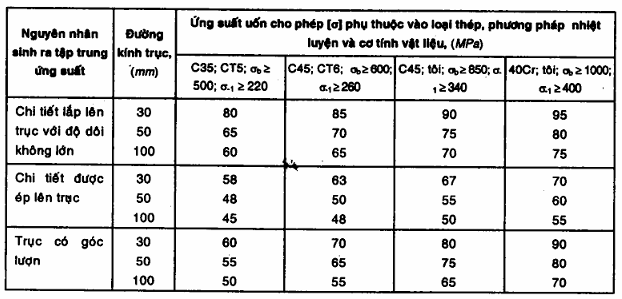
\includegraphics[width=0.8\textwidth]{pictures/bending_stress.png}
                \caption{Ứng suất uốn cho phép}
                \caption*{\footnotesize (Trích tài liệu \cite{gtctm}, trang 403, bảng 10.2)}
            \end{figure}
        \subsection{Chọn kích thước dọc trục}
            \begin{figure}[H]
                \centering
                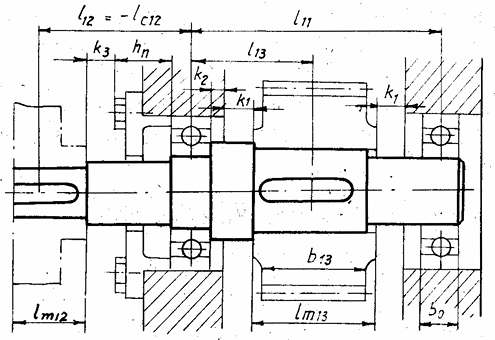
\includegraphics[width=0.75\textwidth]{pictures/shaft.png}
                \caption{Các kích thước dọc trục}
                \label{fig:shaft_standard}
            \end{figure} 
            \hspace*{0.6cm}Chọn các trị số của các thông số liên quan:
            \begin{itemize}
                \item [--] $k_1 = 10 \in (8 \div 15): $ Khoảng cách từ mặt mút của chi tiết quay đến thành trong của hộp.
                \item [--] $k_2 = 10 \in (5 \div 15): $ Khoảng cách từ mặt mút ổ đến thành trong của hộp.
                \item [--] $k_3 = 20 \in (10 \div 20): $ Khoảng cách từ mặt mút của chi tiết quay đến nắp ổ.
                \item [--] $h_n = 25 \in (15 \div 25): $ Chiều cao nắp ổ và đầu bu lông.
            \end{itemize}
            \subsubsection{Trục II}
                \begin{itemize}
                    \item Chiều rộng bánh đai:
                        $$l_{m12} = 44 (mm)$$   
                    \item Chiều dài đoạn $l_{12}$:
                        $$l_{12} = 0.5 \cdot (l_{m12} + b_0) + k_3 + h_n = 0.5 \cdot (44 + 16) + 20 + 25 = 75 (mm)$$
                    \item Chiều dài bánh răng trụ dẫn động:
                        $$l_{m13} = 53 (mm)$$
                    \item Chiều dài đoạn $l_{13}$:
                        $$l_{13} = 0.5 \cdot (l_{m13} + b_0) + k_1 + k_2 = 0.5 \cdot (53 + 16) + 10 + 10 = 54.5 (mm)$$
                    \item Chiều dài đoạn $l_{11}$:
                        $$l_{11} = 2 \cdot l_{13} + 10 = 119 (mm)$$
                    \item Chiều dài trục II:
                        $$l_{II} = l_{11} + l_{12} + 0.5 \cdot l_{m12} = 119 + 75 + 0.5 \cdot 44 = 216 (mm)$$
                \end{itemize}
            \subsubsection{Trục III}
                \begin{itemize}
                    \item Chiều rộng bánh răng côn dẫn động:
                        $$l_{m12} = 86.68 (mm)$$ 
                    \item Chiều dài đoạn $l_{12}$:
                        $$l_{12} = 0.5 \cdot (l_{m12} + b_0) + k_3 + h_n = 0.5 \cdot (86.68 + 29) + 15 + 20 = 92.84 (mm)$$
                    \item Chiều rộng bánh răng trụ bị dẫn:
                        $$l_{m13} = 48 (mm)$$ 
                    \item Chiều dài đoạn $l_{13}$:
                        $$l_{13} = 0.5 \cdot (l_{m13} + b_0) + k_1 + k_2 = 0.5 \cdot (48 + 29) + 10 + 10 = 58.5 (mm)$$
                    \item Chiều dài đoạn $l_{11}$:
                        $$l_{11} = 2 \cdot l_{13} + 16.5 = 133.5 (mm)$$
                    \item Chiều dài trục III:
                        $$l_{III} = l_{11} + l_{12} + 0.5 \cdot l_{m12} = 133.5 + 92.84 + 0.5 \cdot 86.68 = 269.68 (mm)$$
                \end{itemize}
        \subsection{Phân tích lực tác dụng lên trục}
            \subsubsection{Bánh đai bị dẫn}
                \begin{itemize}
                    \item Lực dọc trục bánh đai: $F_d = 813.8\, \mathrm{N}$.
                \end{itemize}
            \subsubsection{Bánh răng trụ 1}
                \begin{itemize}
                    \item Lực vòng bánh răng trụ 1: $F_{t1} = 2845.14 \, \mathrm{N}$.
                    \item Lực dọc trục bánh răng trụ 1: $F_{a1} = 870.39 \, \mathrm{N}$.
                    \item Lực hướng tâm bánh răng trụ 1: $F_{r1} = 1132.59 \, \mathrm{N}$. 
                \end{itemize}
            \subsubsection{Bánh răng trụ 2}
                \begin{itemize}
                    \item Lực vòng bánh răng trụ 2: $F_{t2} = 2845.11\, \mathrm{N}$.
                    \item Lực dọc trục bánh răng trụ 2: $F_{a2} = 870.39\, \mathrm{N}$.
                    \item Lực hướng tâm bánh răng trụ 2: $F_{r2} = 1132.59\, \mathrm{N}$. 
                \end{itemize}
            \subsubsection{Bánh răng côn 1}
                \begin{itemize}
                    \item Lực vòng bánh răng côn 1: $F_{t3} = 10091.75\, \mathrm{N}$.       
                    \item Lực dọc trục bánh răng côn 1: $F_{a3} = 603.71\, \mathrm{N}$.
                    \item Lực hướng tâm bánh răng côn 1: $F_{r3} = 3623.14\, \mathrm{N}$. 
                \end{itemize}
            \newpage
        \subsection{Vẽ biểu đồ momen uốn và xoắn}
            \subsubsection{Vẽ biểu đồ momen uốn và xoắn trục II}
                \begin{figure}[H]
                    \centering
                    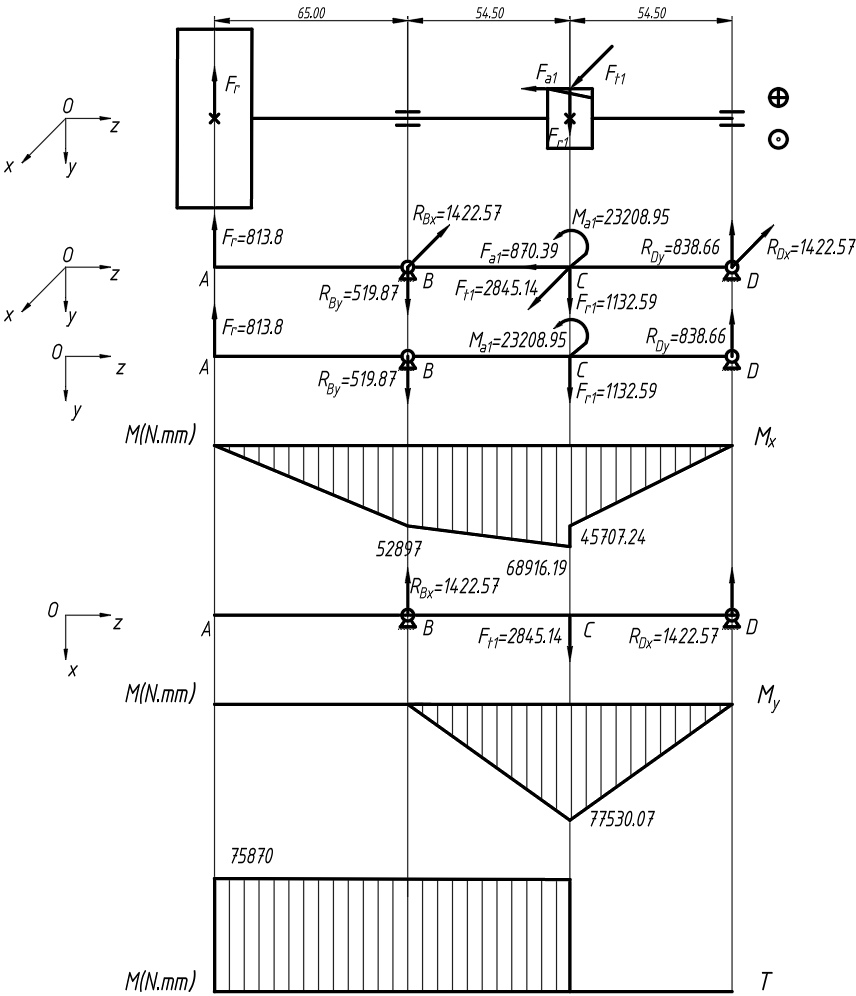
\includegraphics[width = 1\textwidth]{pictures/momen_II.png}
                    \caption{Biểu đồ momen trục II}
                    \label{fig:momen_II}
                \end{figure}
                \newpage
                \begin{itemize}
                    \item Biểu đồ momen uốn và xoắn như hình \ref{fig:momen_II}:
                    \item Trong mặt phẳng Oyz:
                        \begin{itemize}
                            \item Ta có phương trình cân bằng momen:
                            \begin{align*}
                                &\sum{M_{x/B}} = 0 \\
                                \Leftrightarrow& F_{r} \cdot 65 + F_{r1} \cdot 54.5 - M_{a1} - R_{Dy} \cdot 109 = 0 \\
                                \Leftrightarrow& F_{r} \cdot 65 + F_{r1} \cdot 54.5 - F_{a1} \cdot \frac{d_1}{2} - R_{Dy} \cdot 109 = 0 \\
                                \Leftrightarrow& R_{Dy} = \frac{813.8 \cdot 65 + 1132.59 \cdot 54.5 - 870.39 \cdot \frac{53.33}{2}}{109} = 838.66 \, \mathrm{N}
                            \end{align*}
                            \item Phương trình cân bằng lực theo trục y:
                            \begin{align*}
                                &\sum{F_{y}} = 0 \\
                                \Leftrightarrow& -F_{r} + R_{By} + F_{r1} - R_{Dy} = 0 \\
                                \Leftrightarrow& R_{By} = 838.66 + 813.8 - 1132.59 = 519.87\, \mathrm{N}
                            \end{align*}
                        \end{itemize}
                        \item Trong mặt phẳng Ozx:
                        \begin{itemize}
                            \item Ta có phương trình cân bằng momen:
                            \begin{align*}
                                &\sum{M_{y/B}} = 0 \\
                                \Leftrightarrow& F_{t1} \cdot 71 + R_{Dx} \cdot 132 = 0 \\
                                \Leftrightarrow& R_{Dx} = \frac{2845.11 \cdot 54.5}{109} = 1422.57 \, \mathrm{N}
                            \end{align*}
                            \item Phương trình cân bằng lực theo trục x:
                            \begin{align*}
                                &\sum{F_{x}} = 0 \\
                                \Leftrightarrow& -R_{Bx} + F_{t1} - R_{Dx} = 0 \\
                                \Leftrightarrow& R_{Bx} = 2845.11 - 1422.57 = 1422.57  \, \mathrm{N}
                            \end{align*}
                        \end{itemize}
                \end{itemize}
            \subsubsection{Vẽ biểu đồ momen uốn và xoắn trục III}
                \begin{figure}[H]
                    \centering
                    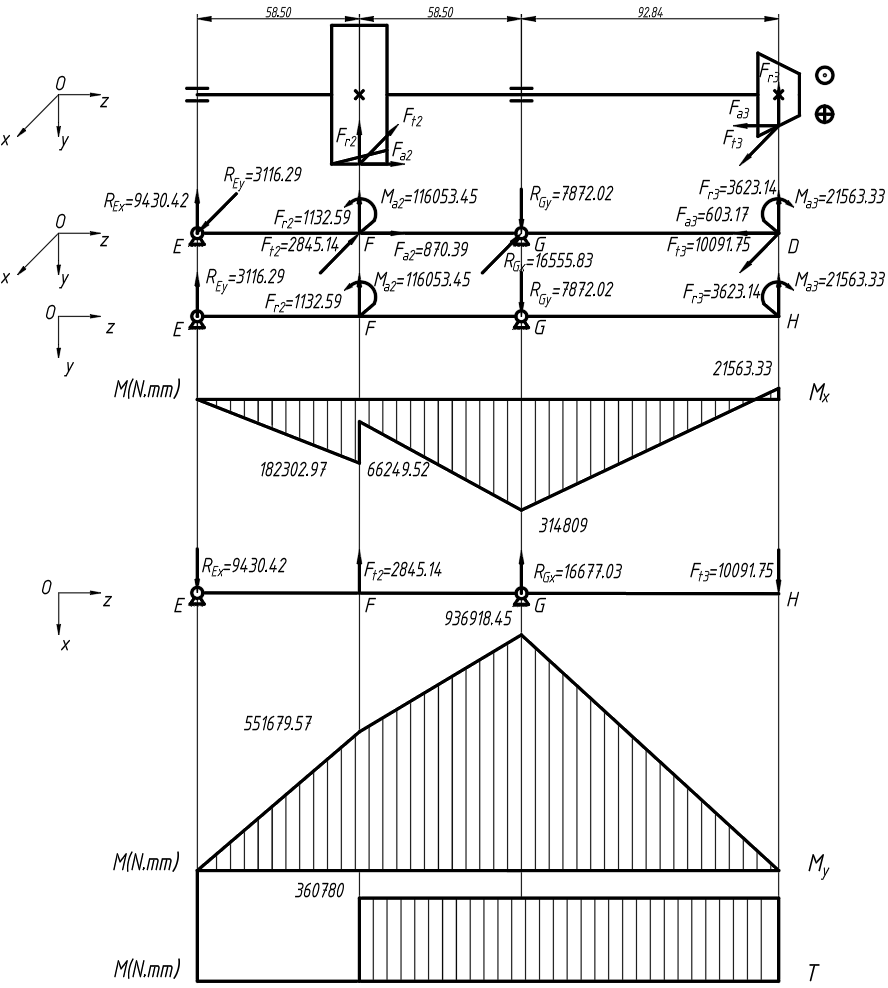
\includegraphics[width = 1.1\textwidth]{pictures/momen_III.png}
                    \caption{Biểu đồ momen trục III}
                    \label{fig:momen_III}
                \end{figure}
                \newpage
                \begin{itemize}
                    \item Biểu đồ momen uốn và xoắn như hình \ref{fig:momen_III}:
                    \item Trong mặt phẳng Oyz:
                        \begin{itemize}
                            \item Ta có phương trình cân bằng momen:
                                \begin{align*}
                                    &\sum{M_{x/E}} = 0 \\
                                    \Leftrightarrow& -F_{r2} \cdot 58.5 - M_{a2} + R_{Gy} \cdot 117 + M_{a3} - F_{r3} \cdot 224.84 = 0 \\
                                    \Leftrightarrow& -F_{r2} \cdot 58.5 - F_{a2} \cdot \frac{d_2}{2} + R_{Gy} \cdot 117 + F_{a3} \cdot \frac{d_3}{2} - F_{r3} \cdot 224.84 = 0 \\
                                    \Leftrightarrow& R_{Gy} = \frac{1132.59 \cdot 58.5 + 870.39 \cdot \frac{266.67}{2} - 603.17 \cdot \frac{71.5}{2} + 3623.14 \cdot 209.84}{117} = 7872.02 \, \mathrm{N}
                                \end{align*}
                            \item Phương trình cân bằng lực theo trục y:
                                \begin{align*}
                                    &\sum{F_{y}} = 0 \\
                                    \Leftrightarrow& R_{Ey} - F_{r2} + R_{Gy} - F_{r3} = 0 \\
                                    \Leftrightarrow& R_{Ey} = - 1132.59 - 3623.14 + 7872.02 = 3116.29 \, \mathrm{N}
                                \end{align*}
                        \end{itemize}
                    \item Trong mặt phẳng Ozx:
                        \begin{itemize}
                            \item Ta có phương trình cân bằng momen:
                                \begin{align*}
                                    &\sum{M_{y/E}} = 0 \\
                                    \Leftrightarrow& -F_{t2} \cdot 58.5 - R_{Gx} \cdot 117 + F_{t3} \cdot 224.84 = 0 \\
                                    \Leftrightarrow& -2845.14 \cdot 58.5 - R_{Gx} \cdot 117 + 10091.75 \cdot 224.84 = 0 \\
                                    \Leftrightarrow& R_{Gx} = \frac{-2845.14 \cdot 58.5 + 10091.75 \cdot 209.84}{117} = 16677.03\, \mathrm{N}
                                \end{align*}
                            \item Phương trinh cân bằng lực theo trục x:
                                \begin{align*}
                                    &\sum{F_{x}} = 0 \\
                                    \Leftrightarrow& R_{Ex} - F_{t2} - R_{Gx} + F_{t3} = 0 \\
                                    \Leftrightarrow& R_{Ex} = 2845.14 + 16677.03 - 10091.75 = 9430.42\, \mathrm{N}
                                \end{align*}
                        \end{itemize}
                \end{itemize}
                    
        \subsection{Xác định momen tương đương và đường kính trục tại tiết diện nguy hiểm}
            \subsubsection{Tính toán trục II}
                \begin{itemize}
                    \item Từ biểu đồ momen ở hình \ref{fig:momen_II} ta thấy rằng tiết diện nguy hiểm nhất của trục II nằm ở vị trí C (bánh răng trụ răng nghiêng dẫn động):
                        \begin{itemize}
                            \item Momen tương đương:
                                \begin{align*}
                                    M_{td} = \sqrt{M_{x}^2 + M_{y}^2 +  0.75T^2} &= \sqrt{68916.19^2 + 77539^2 + 0.75 \cdot 75870^2}\\ 
                                                                                 &= 122790.66 \, \mathrm{N.mm}
                                \end{align*}
                            \item Đường kính trục:
                                \[
                                    d \geq \sqrt[3]{\frac{M_{td}}{0.1 [\sigma]}} = \sqrt[3]{\frac{122790.66}{0.1 \cdot 80}} = 24.85 \, \mathrm{mm}
                                \]
                        \end{itemize}
                        \hspace*{0.6cm}Vì tại điểm C có lắp bánh răng nên có then. Ta tăng đường kính thêm 5\% là $d_C = 26.09 \, \mathrm{mm}$.
                    \item Tính toán các vị trí khác trong trục:
                        \begin{itemize}
                            \item Tại vị trí A (bánh đai bị dẫn):
                                \begin{align*}
                                    M_{td} &= \sqrt{M_{x}^2 + M_{y}^2 +  0.75T^2} = \sqrt{0 + 0 + 0.75 \cdot 75870^2} = 65705.35 \, \mathrm{N.mm}
                                \end{align*}
                                \[
                                    d \geq \sqrt[3]{\frac{M_{td}}{0.1 [\sigma]}} = \sqrt[3]{\frac{65705.35}{0.1 \cdot 80}} = 20.17 \, \mathrm{mm}
                                \]
                                Vì tại điểm A có lắp bánh đai nên có then. Ta tăng đường kính thêm 5\% là $d_A = 21.18 \, \mathrm{mm}$.
                            \item Tại vị trí B và D (ổ lăn), do tại D không chịu momen nên ta tính toán đường kính trục tại ổ lăn theo vị trí B:
                                \begin{align*}
                                    M_{td} &= \sqrt{M_{x}^2 + M_{y}^2 +  0.75T^2} = \sqrt{52897^2 + 0 + 0.75 \cdot 75870^2} = 84352.15 \, \mathrm{N.mm}
                                \end{align*}
                                \[
                                    d \geq \sqrt[3]{\frac{M_{td}}{0.1 [\sigma]}} = \sqrt[3]{\frac{84352.15}{0.1 \cdot 80}} = 21.93 \, \mathrm{mm}
                                \]
                        \end{itemize}
                \end{itemize}
                Ta chọn bộ số đường kính $d_A = 22 \, \mathrm{mm}, d_B = d_D = 30 \, \mathrm{mm}, d_C = 40 \, \mathrm{mm}$. (Do trục có 4 bậc kể cả bậc chứa vòng chắn dầu)
            \subsubsection{Tính toán trục 2 trong hộp giảm tốc (trục III)}
                \begin{itemize}
                    \item Từ biểu đồ momen ở hình \ref{fig:momen_III} ta thấy rằng tiết diện nguy hiểm nhất của trục III nằm ở vị trí G (ổ lăn).
                        \begin{itemize}
                            \item Momen tương đương:
                                \begin{align*}
                                    M_{td} = \sqrt{M_{x}^2 + M_{y}^2 +  0.75T^2} &= \sqrt{314809^2 + 936918.45^2 + 0.75 \cdot 360780^2} \\
                                                                                 &= 1036601.44 \, \mathrm{N.mm}
                                \end{align*}
                            \item Đường kính trục:
                                \begin{align*}
                                    d \geq \sqrt[3]{\frac{M_{td}}{0.1 [\sigma]}} = \sqrt[3]{\frac{1036601.44}{0.1 \cdot 70}} = 52.91\, \mathrm{mm}
                                \end{align*} 
                        \end{itemize}
                    \item Tính toán các vị trí khác trong trục:
                        \begin{itemize}
                            \item Tại vị trí F (bánh răng trụ răng nghiêng bị dẫn):
                                \begin{align*}
                                    M_{td} = \sqrt{M_{x}^2 + M_{y}^2 +  0.75T^2} &= \sqrt{182302.97^2 + 551679.57^2 + 0.75 \cdot 360780^2} \\
                                                                                 &= 659701.71 \, \mathrm{N.mm}
                                \end{align*}
                                \[
                                    d \geq \sqrt[3]{\frac{M_{td}}{0.1 [\sigma]}} = \sqrt[3]{\frac{659701.71}{0.1 \cdot 80}} = 43.52 \, \mathrm{mm}
                                \]
                                Vì tại điểm E có lắp bánh răng nên có then. Ta tăng đường kính thêm 5\% là $d_E = 45.7 \, \mathrm{mm}$.
                            \item Tại vị trí H (bánh răng côn dẫn động):
                                \begin{align*}
                                    M_{td} = \sqrt{M_{x}^2 + M_{y}^2 +  0.75T^2} = \sqrt{21563.33^2 + 0 + 0.75 \cdot 360780^2} = 313187.86 \, \mathrm{N.mm}
                                \end{align*}
                                \[
                                    d \geq \sqrt[3]{\frac{M_{td}}{0.1 [\sigma]}} = \sqrt[3]{\frac{313187.86}{0.1 \cdot 80}} = 33.96 \, \mathrm{mm}
                                \]
                        \end{itemize}
                \end{itemize}
            Ta chọn bộ số đường kính $d_E = d_G = 50 \, \mathrm{mm}, d_F = 60 \, \mathrm{mm}, d_H = 42 \, \mathrm{mm}$.             
        \subsection{Phác thảo sơ bộ trục}
            \subsubsection{Phác thảo sơ bộ trục II}
                \begin{figure}[H]
                    \centering
                    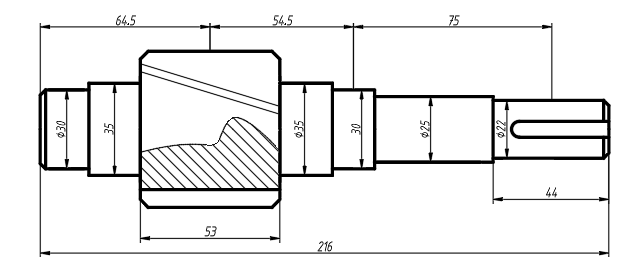
\includegraphics[width=1\textwidth]{pictures/shaft_II.png}
                    \caption{Phác thảo sơ bộ trục II}
                    \label{fig:shaft_II}
                \end{figure}
            \subsubsection{Phác thảo sơ bộ trục III}
               \begin{figure}[H]
                    \centering
                    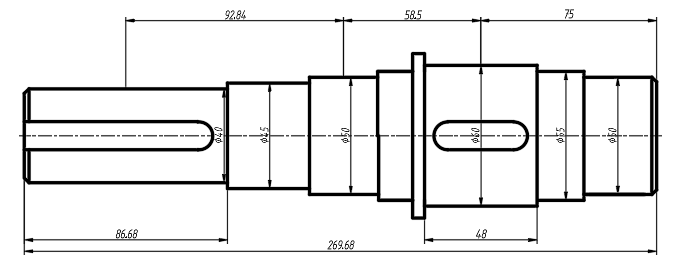
\includegraphics[width=1\textwidth]{pictures/shaft_III.png}
                    \caption{Phác thảo sơ bộ trục III}
                    \label{fig:shaft_III}
                \end{figure}
    \section{Thiết kế mối ghép then}
        \subsection{Tính mối ghép then}
            \begin{figure}[H]
                \centering
                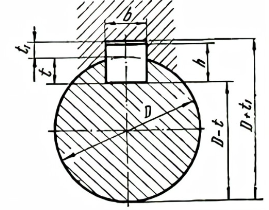
\includegraphics[width=0.4\textwidth]{pictures/key.png}
                \caption{Mối ghép then}
                \label{fig:key}
            \end{figure}
            \begin{itemize}
                \item Do các trục đều nằm trong hộp giảm tốc nên ta chọn then bằng. Để đảm bảo tính công nghệ, chọn then giống nhau trên cùng 1 trục.
                    \begin{figure}[H]
                        \centering
                        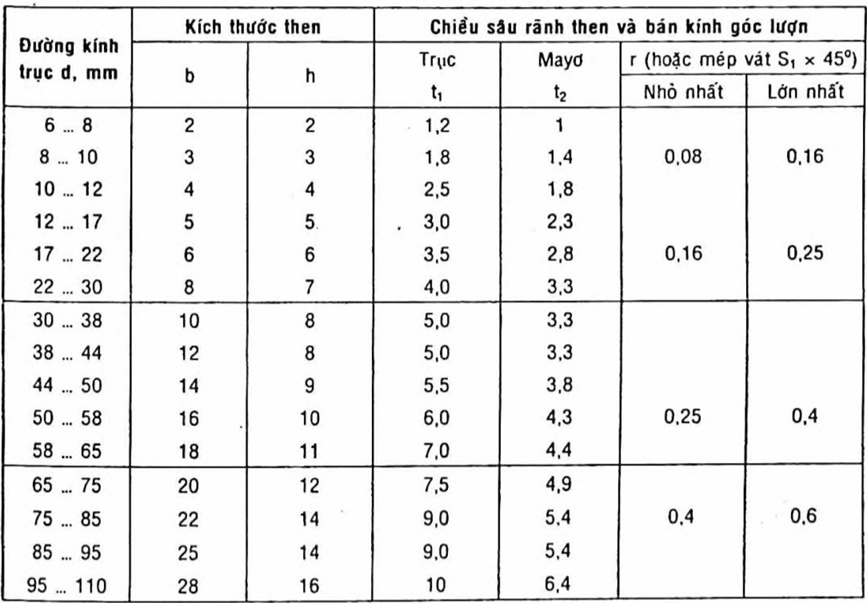
\includegraphics[width=0.8\textwidth]{pictures/key_standard.png}
                        \caption{Tiêu chuẩn về mối ghép then bằng}
                        \label{fig:key_standard}
                        \caption*{\footnotesize (Trích tài liệu \cite{btctm}, trang 188, phụ lục 13.1)}
                    \end{figure}
                \item Từ những dữ liệu tính toán được và bảng \ref{fig:key_standard} ta có bảng số liệu về then như sau:
                    \begin{table}[H]
                        \centering
                        \begin{tabular}{|c|c|c|c|c|}
                            \hline
                            \textbf{Tiết diện} & \textbf{d, mm} & \textbf{b x h, mm} & $\mathbf{t_{1}, mm}$ & $\mathbf{t_{2}, mm}$  \\
                            \hline
                            \textbf{Bánh đai bị dẫn} & 22 & 6 x 6 & 3.5 & 2.8  \\
                            \hline
                            \textbf{Bánh răng nghiêng (I)} & 40 & 12 x 8 & 5 & 3.3  \\
                            \hline
                            \textbf{Bánh răng nghiêng (II)} & 60 & 18 x 11 & 7 & 4.4  \\
                            \hline
                            \textbf{Bánh răng côn (I)} & 40 & 12 x 8 & 5 & 3.3  \\
                            \hline
                        \end{tabular}
                        \caption{Bảng số liệu về then}
                    \end{table}
            \end{itemize}

        \subsection{Kiểm nghiệm then}
            \begin{itemize}
                \item Xác định chiều dài các mayơ:
                    \begin{itemize}
                        \item Chiều dài mayơ bánh đai ở trục II:
                            \[
                                l_{m1} = B_{d} = 44 \, \mathrm{mm}
                            \]
                        \item Chiều dài mayơ bánh răng trụ răng nghiêng 1 ở trục II: 
                            \[
                                l_{m2} = B_{1}= 53 \, \mathrm{mm}
                            \]  
                        \item Chiều dài mayơ bánh răng trụ răng nghiêng 2 ở trục III:
                            \[
                                l_{m2} = B_{2}= 48 \, \mathrm{mm}
                            \]
                        \item Chiều dài mayơ bánh răng côn ở trục III:
                            \[
                                l_{m3} = B_{w}= 86.68 \, \mathrm{mm}
                            \]
                    \end{itemize}
                \item Xác định chiều dài then: 
                    \[
                        l_{t} = (0.8...0.9)l_m \footnote{Trích tài liệu \cite{tltk1}, trang 174.}
                    \]
                    \begin{itemize}
                        \item Chiều dài then bánh đai ở trục II:
                            \[
                                l_{t0} = (0.8...0.9)l_{m1} = (0.8...0.9) \cdot 44 = 35.2...39.6 \, \mathrm{mm}
                            \]
                            $\Rightarrow$ Theo tiêu chuẩn ta chọn $l_{t0} = 40 \, \mathrm{mm}$
                        \item Chiều dài then bánh răng trụ răng nghiêng 1 ở trục II: 
                            \[
                                l_{t1} = (0.8...0.9)l_{m2} = (0.8...0.9) \cdot 53 = 42.4...47.7 \, \mathrm{mm}
                            \]
                            $\Rightarrow$ Theo tiêu chuẩn ta chọn $l_{t1} = 45 \, \mathrm{mm}$
                        \item Chiều dài then bánh răng trụ răng nghiêng 2 ở trục III:
                            \[
                                l_{t2} = (0.8...0.9)l_{m2} = (0.8...0.9) \cdot 48  = 38.4...43.2  \, \mathrm{mm}
                            \]
                            $\Rightarrow$ Theo tiêu chuẩn ta chọn $l_{t2} = 40 \, \mathrm{mm}$
                        \item Chiều dài then bánh răng côn ở trục III:
                            \[
                                l_{t3} = (0.8...0.9)l_{m3} = (0.8...0.9) \cdot 86.68 = 69.34...78.01 \, \mathrm{mm}
                            \]
                            $\Rightarrow$ Theo tiêu chuẩn ta chọn $l_{t3} = 80 \, \mathrm{mm}$
                    \end{itemize}
                \item Kiểm tra then:
                    \begin{figure}[H]
                        \centering
                        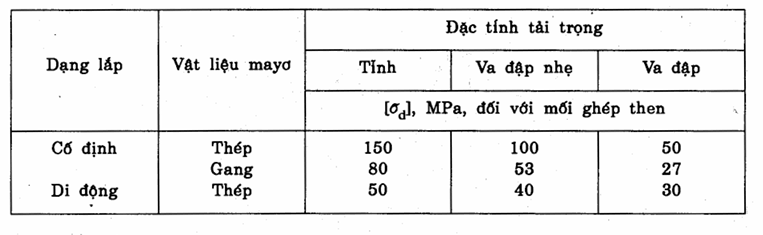
\includegraphics[width=0.8\textwidth]{pictures/key_check.png}
                        \caption{Ứng suất dập cho phép $\sigma_{d}$ đối với mối ghép then}
                        \caption*{\footnotesize (Trích tài liệu \cite{tltk1}, trang 178, bảng 9.5)}
                        \label{fig:key_check}
                    \end{figure}
                    \begin{itemize}
                        \item Do đặc tính tải trọng là tĩnh và dạng lắp là cố địng. Vật liệu mayơ làm bằng thép nên ứng suất dập cho phép $\sigma_{d} = 150 \, \mathrm{MPa}$.
                        \item Tính toán ứng suất dập:
                            \[
                                \sigma_{d} = \frac{2T \cdot 10^3}{t_{2} \cdot d \cdot l_{l}} \footnote{Trích tài liệu \cite{gtctm}, trang 623, công thức 16.1.}
                            \]
                            Trong đó: $l_{l} = l - b \, \mathrm{mm}$.
                        \item Ta có bảng số liệu về tính toán then:
                            \begin{table}[H]
                                \centering
                                \begin{tabular}{|c|c|c|c|c|c|}
                                    \hline
                                    \textbf{Tiết diện} & \textbf{d, mm} & \textbf{b x h x l, mm} & \textbf{T, Nm} & $\mathbf{t_{2}, mm}$ & $\mathbf{\sigma_{d}, MPa}$ \\
                                    \hline
                                    \textbf{Bánh đai bị dẫn} & 22 & 6 x 6 x 40  & 75.87 & 3.5 & 57.96  \\
                                    \hline
                                    \textbf{Bánh răng nghiêng (I)} & 40 & 12 x 8 x 45 & 75.87 & 5 & 22.99  \\
                                    \hline
                                    \textbf{Bánh răng nghiêng (II)} & 60 & 18 x 11 x 40 & 360.78 & 7 & 78.09  \\
                                    \hline
                                    \textbf{Bánh răng côn (I)} & 40 & 12 x 8 x 80 & 360.78 & 5 & 53.05 \\
                                    \hline
                                \end{tabular}
                                \caption{Bảng số liệu về then}
                            \end{table}
                            $\Rightarrow$ Điều kiện bền dập của cả 4 then đều thỏa mãn $\sigma_{d} < [\sigma_{d}]$. Then bằng được chọn theo tiêu chuẩn nên không cần thiết kiểm tra theo độ bền cắt.
                    \end{itemize}
                    \hspace*{0.6cm}Vì đường kính trục tại tiết diện lắp bánh răng nghiêng I là $40 (mm)$ và đường kính chân răng là $45.33 (mm)$. Khi đó khoảng cách từ đỉnh then đến chân răng $ = \frac{45.33 - 40}{2} - t_1 = -0.835 (mm)$ $\rightarrow$ Ta thiết kế bánh răng liền trục tại vị trí C và không lắp then.
            \end{itemize}
    \section{Kiểm nghiệm trục}
        \hspace*{0.6cm}Kết cấu trục vừa thiết kế đảm bảo được độ bền mỏi nếu hệ số an toàn tại các tiết diện nguy hiểm thỏa mãn điều kiện sau:
        $$s_j = \frac{s_{\sigma j}s_{\tau j}}{\sqrt{s^2_{\sigma j}+ s^2_{\tau j}}} \geq [s]$$
        Trong đó:
        \begin{itemize}
            \item[] $[s]$: Hệ số an toàn cho phép. Theo \textit{trang 195 tài liệu tham khảo \cite{tltk1}}, chọn $[s] = 3$ thì không cần kiểm nghiệm về độ cứng của trục.
            \item[] $s_{\sigma j}, s_{\tau j}$: Hệ số an toàn chỉ xét riêng ứng suất pháp và hệ số an toàn chỉ xét riêng ứng suất tiếp tại tiết diện j:
            \begin{align*}
                &s_{\sigma j} = \frac{\sigma_{-1}}{K_{\sigma dj}\sigma_{aj} + \psi_\sigma \sigma_{mj}} \\
                &s_{\tau j} = \frac{\tau_{-1}}{K_{\tau dj}\tau_{aj} + \psi_\tau \tau_{mj}}
            \end{align*}
            Trong đó:
            \begin{itemize}
                \item[--] $\sigma_{-1}, \tau_{-1}$: Giới hạn mỏi uốn và xoắn ứng với chu kỳ đối xứng.Theo \textit{trang 196 tài liệu tham khảo \cite{tltk1}}, lấy gần đúng $\sigma_{-1} = 0.436 \cdot \sigma_b = 0.436.850 = 370.6 (MPa)$ và $\tau_{-1} = 0.58 \cdot \sigma_{-1} = 0.58 \cdot 370.6 = 214.95 (MPa)$ vì vật liệu làm trục - Thép C45 là thép Carbon trung bình.
                \item[--] $\sigma_{aj}, \tau_{aj}, \sigma_{mj}, \tau_{mj}$: Biên độ và trị số trung bình của ứng suất pháp và ứng suất tiếp tại tiết diện j. Xét cho cả hai trục, ta đều có các tính chất sau:
                \begin{itemize}
                    \item[+] Đối với trục quay, ứng suất uốn thay đổi theo chu kỳ đối xứng:
                    $$\sigma_{mj} = 0; \sigma_{aj} = \frac{M_j}{W_j}$$
                    \item[+] Đối với trục quay 1 chiều, ứng suất xoắn tay đổi theo chu kỳ mạch động
                    $$\tau_{mj} = \tau_{aj} = \frac{T_j}{2W_{oj}}$$
                    Trong đó, $W_j, W_{oj}$ là momen cản uốn và momen cản xoắn tại tiết diện j của trục, được xác định theo \textit{bảng 10.6 tài liệu tham khảo \cite{tltk1}}. Vì trục II có 1 rãnh then và trục III có 2 rãnh then:
                    \begin{align*}
                        &W_{II} = \frac{\pi d_j^3}{32} - \frac{bt_1(d_j - t_1)^2}{2 \cdot d_j}\\
                        &W_{oII} = \frac{\pi d_j^3}{16} - \frac{bt_1(d_j - t_1)^2}{2 \cdot d_j}\\
                        &W_{III} = \frac{\pi d_j^3}{32} - \frac{bt_1(d_j - t_1)^2}{d_j}\\
                        &W_{oIII} = \frac{\pi d_j^3}{16} - \frac{bt_1(d_j - t_1)^2}{d_j}
                    \end{align*}
                \end{itemize}
                \item[--] $\psi_\sigma, \psi_\tau$: Hệ số kể đến ảnh hưởng của trị số ứng suất trung bình đến độ bền mỏi, theo \textit{bảng 10.7 tài liệu tham khảo [2]}. 
                \item[--] $K_{\sigma dj}, K_{\tau dj}$: Hệ số, được xác định theo:
                \begin{align*}
                    &K_{\sigma dj} = \frac{K_\sigma/\epsilon_\sigma + K_x - 1}{K_y}\\
                    &K_{\tau dj} = \frac{K_\tau/\epsilon_\tau + K_x - 1}{K_y}
                \end{align*}
                Trong đó:
                \begin{itemize}
                    \item[+] $K_x$: Hệ số tập trung ứng suất do trạng thái bề mặt, phụ thuộc vào phương pháp gia công và độ nhẵn bề mặt, cho trong \textit{bảng 10.8 tài liệu tham khảo \cite{tltk1}}.
                    \item[+] $K_y$: Hệ số tăng bền bề mặt trục, phụ thuộc vào phương pháp tăng bền bề mặt và cơ tính vật liệu, cho trong\textit{ bảng 10.9 tài liệu tham khảo \cite{tltk1}}.
                    \item[+] $\epsilon_\sigma, \epsilon_\tau$: Hệ số kích thước kể đến ảnh hưởng của kích thước tiết diện trục đến giới hạn mỏi, cho trong \textit{bảng 10.10 tài liệu tham khảo \cite{tltk1}}
                    \item[+] $K_\sigma, K_\tau$: Hệ số tập trung ứng suất thực tế khi uốn và khi xoắn, trị số của chúng phụ thuộc vào loại yếu tố gây tập trung ứng suất, cho trong \textit{bảng 10.11 tài liệu tham khảo \cite{tltk1}}.
                \end{itemize}
            \end{itemize}
    \end{itemize}
    \begin{table}[H]
        \centering
        \begin{tabular}{|c|c|c|}
            \hline
            \diagbox{\textbf{Thông số}}{\textbf{Trục}}  & \textbf{Trục II} & \textbf{Trục III} \\ \hline
            $\sigma_{-1} (\, \mathrm{MPa})$ & \multicolumn{2}{c|}{370.6}\\ \hline
            $\tau_{-1} (\, \mathrm{MPa})$ & \multicolumn{2}{c|}{214.95}\\ \hline
            $d$ & 40 & 55\\ \hline
            $b$ & 10 & 16 \\ \hline
            $t_1$ & 5 & 6 \\ \hline
            $\sigma_{mj} (\, \mathrm{MPa})$ & \multicolumn{2}{c|}{0} \\ \hline
            $\sigma_{aj} (\, \mathrm{MPa})$ & 22.09 & 85.81 \\ \hline
            $\tau_{mj} = \tau_{aj} (\, \mathrm{MPa})$ & 3.21 & 6.33 \\ \hline
            $W_j$ & 5517.56 & 12142.99 \\ \hline
            $W_{oj}$ & 11800.75 & 28476.82\\ \hline
            $M (\, \mathrm{N.mm})$ & 121914.81 & 1041993.85 \\ \hline
            $T (\, \mathrm{N.mm})$ & 75870 & 360780 \\ \hline
            $\psi_{\sigma}$ &  \multicolumn{2}{c|}{$0.1$} \\ \hline
            $\psi_{\tau}$ &  \multicolumn{2}{c|}{$0.05$} \\ \hline
            $K_{x}$ & \multicolumn{2}{c|}{1} \\ \hline
            $K_{y}$ &  \multicolumn{2}{c|}{2.5} \\ \hline
            $\epsilon_\sigma$ & 0.85 & 0.8 \\ \hline
            $\epsilon_\tau$ & 0.78 & 0.75 \\ \hline
            $K_{\sigma}$ & \multicolumn{2}{c|}{$2.07$} \\ \hline
            $K_{\tau}$ & \multicolumn{2}{c|}{$1.97$} \\ \hline
            $K_{\sigma dj}$ & 0.974 & 1.04 \\ \hline
            $K_{\tau dj}$ & 1.01 & 1.05 \\ \hline
            $s_{\sigma j}$ & 17.22 & 4.15 \\ \hline
            $s_{\tau j}$ & 63.17 & 30.87 \\ \hline
            $s_j$ & 16.61 & 4.11 \\ \hline
        \end{tabular}
        \caption{Bảng thông số bộ truyền bánh răng trụ răng nghiêng}
    \end{table}
    $\rightarrow$ Cả hai trục đều đảm bảo được độ bền mỏi, không cần kiểm nghiệm về độ bền cứng.
    
                    
            
            
        \chapter{THIẾT KẾ Ổ LĂN}
    \section{THIẾT KẾ Ổ TRÊN TRỤC II}
        \subsection{Phân tích lực tác dụng lên ổ}
            \begin{figure}[H]
                \centering
                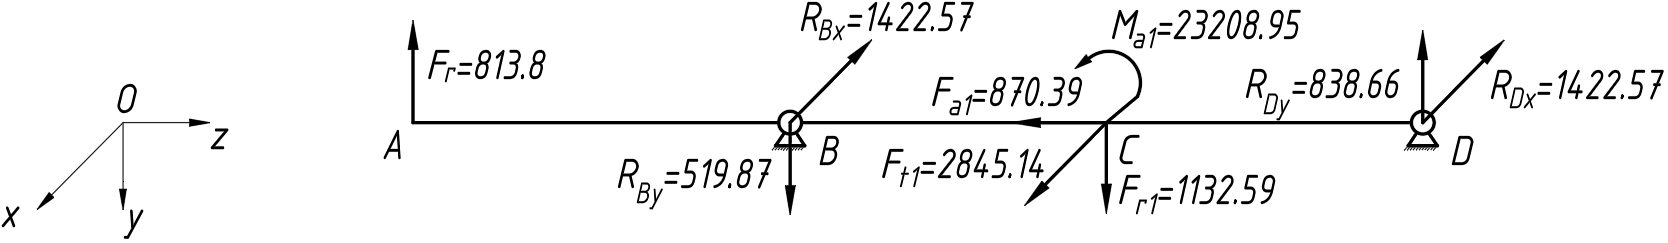
\includegraphics[width=1\textwidth]{pictures/bearing_II.png}
                \caption{Lực tác dụng lên ổ trục II}
            \end{figure}
            \subsubsection{Xác định phản lực tác dụng lên ổ}
                \[
                    F_{r} = \sqrt{F_{rx}^2 + F_{ry}^2} = \sqrt{R_{x}^2 + R_{y}^2}\footnote{Trích tài liệu \cite{gtctm}, trang 442, công thức 11.17}
                \]
                \begin{itemize}
                    \item Phản lực tác dụng lên ổ B:
                        \begin{align*}
                            F_{rB} &= \sqrt{R_{Bx}^2 + R_{By}^2} = \sqrt{1314.8^2 + 586.21^2} = 1439.56\, \mathrm{N}
                        \end{align*}
                    \item Phản lực tác dụng lên ổ D:
                        \begin{align*}
                            F_{rD} &= \sqrt{R_{Dx}^2 + R_{Dy}^2} = \sqrt{1530.34^2 + 905^2} = 1777.91\, \mathrm{N}
                        \end{align*}
                \end{itemize}
                \hspace*{0.6cm}Vì $F_{rB} < F_{rD}$ nên ta sẽ tính toán chọn ổ lăn theo ổ lăn D. $F_{r} = F_{rD} = 1777.91\, \mathrm{N}$
            \subsubsection{Xác định lực dọc trục tác dụng lên ổ}
                \begin{align*}
                    F_{a} = F_{a1} = 870.39\, \mathrm{N}
                \end{align*}
        \subsection{Chọn sơ bộ ổ lăn}
            \begin{figure}[H]
                \centering
                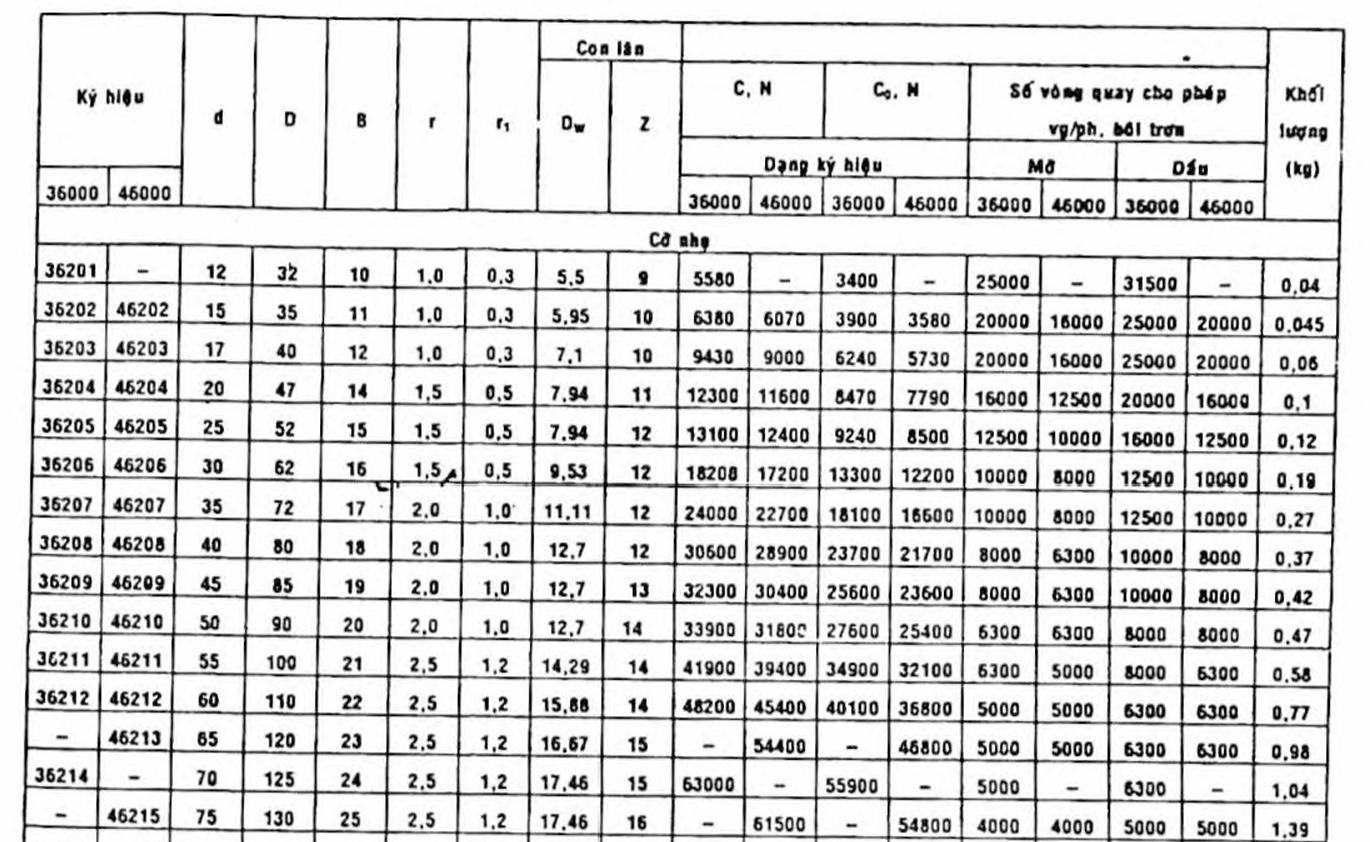
\includegraphics[width=1\textwidth]{pictures/bearing_standard_II.png}
                \caption{Tiêu chuẩn ổ đỡ chặn}
                \caption*{\footnotesize(Trích tài liệu \cite{btctm}, trang 512, phụ lục 9.3)}
            \end{figure}
            \begin{itemize}
                \item Ta có: $0.3 \leq \frac{F_a}{F_r} = \frac{870.39}{1777.91} = 0.489 \leq 0.7$. \\[0.3cm]
                    $\Rightarrow$ Chọn loại ổ là ổ bi đỡ chặn 1 dãy.
                \item Ta có đường kính trục tại ổ lăn: $d = d_{B} = d_{D} = 30\, \mathrm{mm}$
                \item Chọn ổ lăn là ổ bi đỡ chặn, cỡ nhẹ có ký hiệu 36206  $(\alpha = 12 ^\circ)$ với $C = 18208\, \mathrm{N}$ và $C_o = 13300\, \mathrm{N}$.
                \item Chọn cấp chính xác cho ổ lăn là 0. Có độ đảo hướng tâm $20\, \mathrm{\mu m}$. Giá thành tương đối là 1.
            \end{itemize}
        \subsection{Tính ổ lăn theo khả năng tải động}
            \subsubsection{Chọn các hệ số}
                \begin{itemize}
                    \item Chọn hệ số $K_{\sigma} = 1$ do tải trọng tỉnh.
                    \item Chọn hệ số $K_{t} = 1$ do làm việc ở nhiệt độ bình thường.
                    \item Chọn hệ số $V = 1$ do vòng trong quay.
                    \item Chọn hệ số X và Y:
                        \begin{itemize}
                            \item Tỉ số $\frac{F_{a}}{C_{o}} = \frac{870.39}{13300} = 0.065 \Rightarrow$ Chọn $e = 0.38$.
                            \item Tỉ số $\frac{F_{a}}{VF_{r}} = \frac{870.39}{1 \cdot 1777.91} = 0.49 > e \Rightarrow$ Chọn $X = 0.45$ và $Y = 1.45$.
                        \end{itemize}
                \end{itemize}
            \subsubsection{Tính khả năng tải động}
                \begin{itemize}
                    \item Thời gian làm việc tính bằng triệu vòng quay:
                        \[
                            L = \frac{60nL_{h}}{10^6}\footnote{Trích tài liệu \cite{gtctm}, trang 449, công thức 11.25b} = \frac{60 \cdot 360 \cdot 24000}{10^6} = 518.4\, \textrm{triệu vòng} 
                        \]
                    \item Tải trọng quy ước tác dụng lên ổ lăn:
                        \[
                            Q = Q_{r} = (XVF_{r} + YF_{a}) \cdot K_{\sigma}K_{t} \footnote{Trích tài liệu \cite{gtctm}, trang 444, công thức 11.20} = (0.45 \cdot 1 \cdot 1777.91 + 1.45 \cdot 870.39) \cdot 1 \cdot 1 = 2062.13\, \mathrm{N}
                        \]
                    \item Khả năng tải động tính toán của ổ:
                        \[
                            C_{tt} = Q \cdot \sqrt[m]{L} \footnote{Trích tài liệu \cite{gtctm}, trang 450, công thức 11.27} = 2062.13 \cdot \sqrt[3]{518.4} = 16565.49\, \mathrm{N}
                        \
                        \]
                        Ta có: $C_{tt} = 16065.49\, \mathrm{N} < C = 18208\, \mathrm{N}$ $\Rightarrow$ Thỏa điều kiện tải tĩnh.
                \end{itemize}
                \begin{table}[H]
                    \centering
                    \begin{tabular}{|c|c|c|c|c|c|c|c|c|c|}
                        \hline
                        \textbf{Ký hiệu} & \textbf{d, mm} & \textbf{D, mm} & \textbf{B, Nm} & \textbf{r, mm} & $\mathbf{r_{1}, mm}$ & $\mathbf{C, N}$ & $\mathbf{C_{o}, N}$ & $\mathbf{L_{h}}$, \textbf{giờ} \\
                        \hline
                        36206 & 30 & 62 & 16 & 1.5 & 0.5 & 18208 & 13300 & 24000 \\
                        \hline
                    \end{tabular}
                    \caption{Bảng số liệu về con lăn trục II}
                \end{table}
    \section{THIẾT KẾ Ổ TRÊN TRỤC III}
        \subsection{Phân tích lực tác dụng lên ổ}
            \begin{figure}[H]
                \centering
                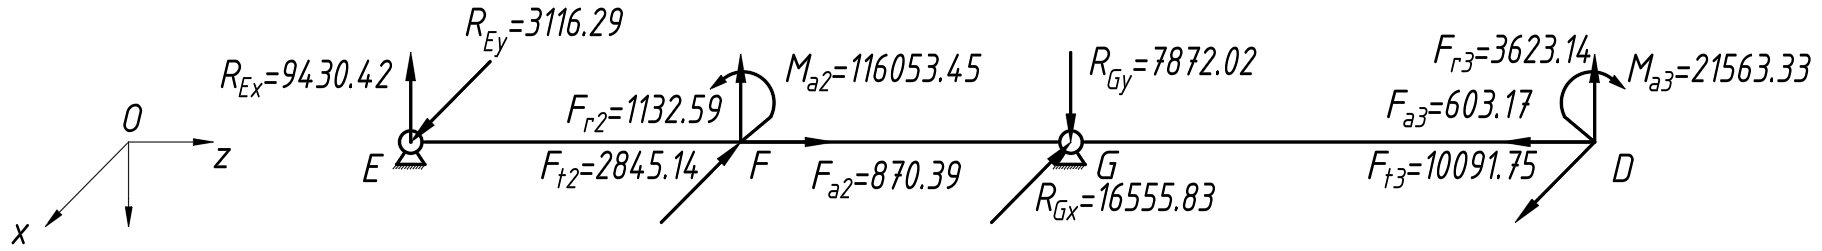
\includegraphics[width=1\textwidth]{pictures/bearing_III.png}
                \caption{Lực tác dụng lên ổ trục III}
            \end{figure}
            \subsubsection{Xác định phản lực tác dụng lên ổ}
                \[
                    F_{r} = \sqrt{F_{rx}^2 + F_{ry}^2} = \sqrt{R_{x}^2 + R_{y}^2}
                \]
                \begin{itemize}
                    \item Phản lực tác dụng lên ổ E:
                        \begin{align*}
                            F_{rE} &= \sqrt{R_{Ex}^2 + R_{Ey}^2} = \sqrt{9309.2^2 + 2924.38^2} = 9757.72\, \mathrm{N}
                        \end{align*}
                    \item Phản lực tác dụng lên ổ G:
                        \begin{align*}
                            F_{rG} &= \sqrt{R_{Gx}^2 + R_{Gy}^2} = \sqrt{16555.83^2 + 7680.11^2} = 18250.47\, \mathrm{N}
                        \end{align*}
                \end{itemize}
                \hspace*{0.6cm}Vì $F_{rE} < F_{rG}$ nên ta sẽ tính toán chọn ổ lăn theo ổ lăn G. $F_{r} = F_{rG} = 18250.47\, \mathrm{N}$
            \subsubsection{Xác định lực dọc trục tác dụng lên ổ}
                \begin{align*}
                    F_{a} = |F_{a2} - F_{a3}| = |870.39 - 603.17| = 267.22\, \mathrm{N}
                \end{align*}
        \subsection{Chọn sơ bộ ổ lăn}
            \begin{figure}[H]
                \centering
                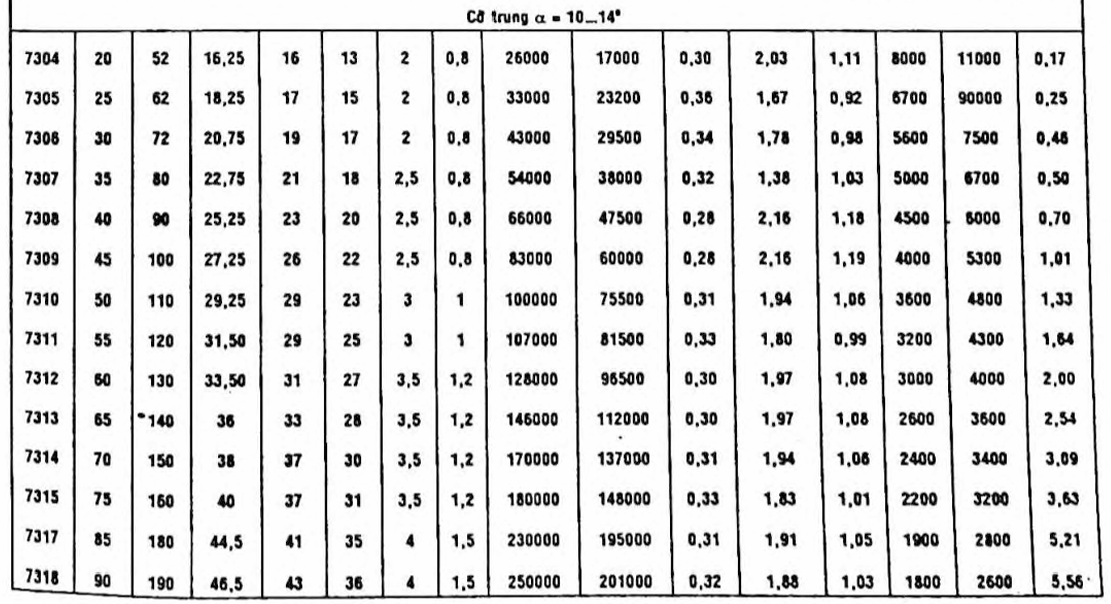
\includegraphics[width=1\textwidth]{pictures/bearing_standard_III.png}
                \caption{Tiêu chuẩn ổ đũa côn}
                \caption*{\footnotesize(Trích tài liệu \cite{btctm}, trang 512, phụ lục 9.3)}
            \end{figure}
            \begin{itemize}
                \item Ta có: $\frac{F_a}{F_r} = \frac{267.22}{18250.47} = 0.015 \leq 0.3$. \\[0.3cm]
                Để đảm bảo độ cứng ổ cao ta chọn loại ổ là ổ đũa côn.
                \item Ta có đường kính trục tại ổ lăn: $d = d_{E} = d_{G} = 50\, \mathrm{mm}$
                \item Chọn ổ lăn là ổ đũa côn, cỡ trung có ký hiệu 7310 với $C = 100000\, \mathrm{N}$ và $C_o = 75500\, \mathrm{N}$.
                \item Chọn cấp chính xác cho ổ lăn là 0. Có độ đảo hướng tâm $20\, \mathrm{\mu m}$. Giá thành tương đối là 1.
            \end{itemize}
        \subsection{Tính ổ lăn theo khả năng tải động}
            \subsubsection{Chọn các hệ số}
                \begin{itemize}
                    \item Chọn hệ số $K_{\sigma} = 1$ do tải trọng tỉnh.
                    \item Chọn hệ số $K_{t} = 1$ do làm việc ở nhiệt độ bình thường.
                    \item Chọn hệ số $V = 1$ do vòng trong quay.
                    \item Chọn hệ số X và Y:
                        \begin{itemize}
                            \item Tỉ số $\frac{F_{a}}{C_{o}} = \frac{267.22}{75500} = 0.003 \Rightarrow$ Chọn $e = 0.3$.
                            \item Tỉ số $\frac{F_{a}}{VF_{r}} = \frac{267.22}{1 \cdot 18250.47} = 0.015 < e \Rightarrow$ Chọn $X = 1$ và $Y = 0$.
                        \end{itemize}
                \end{itemize}
            \subsubsection{Tính khả năng tải động}
                \begin{itemize}
                    \item Thời gian làm việc tính bằng triệu vòng quay:
                        \[
                            L = \frac{60nL_{h}}{10^6} = \frac{60 \cdot 72 \cdot 24000}{10^6} = 103.68\, \textrm{triệu vòng} 
                        \]
                    \item Tải trọng quy ước tác dụng lên ổ lăn:
                        \[
                            Q = Q_{r} = (XVF_{r} + YF_{a}) \cdot K_{\sigma}K_{t} = (1 \cdot 1 \cdot 18250.47 + 0 \cdot 267.22) \cdot 1 \cdot 1 = 18250.47\, \mathrm{N}
                        \]
                    \item Khả năng tải động tính toán của ổ:
                        \[
                            C_{tt} = Q \cdot \sqrt[m]{L} = 18250.47 \cdot \sqrt[3]{103.68} = 85737 \, \mathrm{N}
                        \]
                        Ta có:  $C_{tt} = 85737\, \mathrm{N} < C = 100000\, \mathrm{N}$ $\Rightarrow$ Thỏa điều kiện tải tĩnh. 
                \end{itemize} 
                \begin{table}[H]
                    \centering
                    \begin{tabular}{|c|c|c|c|c|c|c|c|c|}
                        \hline
                        \textbf{Ký hiệu} & \textbf{d, mm} & \textbf{D, mm} & \textbf{B, Nm} & \textbf{r, mm} & $\mathbf{C, N}$ & $\mathbf{C_{o}, N}$ & $\mathbf{L_{h}}$, \textbf{giờ} \\
                        \hline
                        7310 & 50 & 110 & 29 & 3 & 100000 & 75500 & 24000 \\
                        \hline
                    \end{tabular}
                    \caption{Bảng số liệu về con lăn trục III}
                \end{table}

                    
                
            
        \chapter{CHỌN THÂN MÁY, BULÔNG VÀ CÁC CHI TIẾT KHÁC}
    \section{TÍNH TOÁN VỎ HỘP}
        \begin{longtable}{|p{7.5cm}|p{8.3cm}|}
            \hline
            \textbf{Tên gọi} & \textbf{Biểu thức tính toán} \\
            \hline
            Chiều dày: & \\
            - Thân hộp, $\delta$ & $\delta = 10$ (mm) \\
            - Nắp hộp, $\delta_1$ & $\delta_1 = 8$ (mm) \\
            \hline
            Gân tăng cứng: & \\
            - Chiều dày, $e$ & $e = 10$ (mm) \\
            - Chiều cao, $h$ & $h = 103$ (mm) \\
            - Độ dốc & $6:1$ \\
            \hline
            Đường kính: & \\
            - Bu lông nền, $d_1$ & $d_1 > 0.04a + 10 > 12, d_1 = 16$ (mm) \\
            - Bu lông cạnh ổ, $d_2$ & $d_2 = (0.7 \div 0.8)d_1 = 14$ (mm) \\
            - Bu lông ghép bích nắp và thân, $d_3$ & $d_3 = (0.8 \div 0.9)d_2 = 10$ (mm) \\
            - Vít ghép nắp ổ, $d_4$ & $d_4 = (0.6 \div 0.7)d_2 = 10$ (mm) \\
            - Vít ghép nắp cửa thăm dò, $d_5$ & $d_5 = (0.5 \div 0.6)d_2 = 6$ (mm) \\
            \hline
            Mặt bích ghép nắp và thân: & \\
            - Chiều dày bích thân hộp, $s_1$ & $s_1 = (1.4 \div 1.8)d_3 = 18$ (mm) \\
            - Chiều dày bích nắp hộp, $s_2$ & $s_2 = (0.9 \div 1)s_3 = 15$ (mm) \\
            - Bề rộng bích nắp và thân, $S_1$ & $S_1 = 43$ (mm) \\
            - Bề rộng mặt bích ổ đỡ, $S_2$ & $S_2 = 52$ (mm) \\
            - Bề rộng mặt đế hộp, $S_3$ & $S_3 = 60$ (mm) \\
            \hline
            Kích thước gối trục: & \\
            - Khoảng cách từ tâm bu lông $d_2$ đến thành trong ổ: $C$ & $C = 37$ (mm) \\
            - Bề rộng mặt ghép bu lông cạnh ổ, $K$ & $K = 50$ (mm) \\
            - Chiều cao h. & Phụ thuộc tâm lỗ bu lông và kích thước mặt tựa. \\
            \hline
            \pagebreak    
            \hline
            Khe hở giữa các chi tiết & \\
            - Giữa bánh răng với thành trong hộp & $\Delta \geq (1 \div 1,2)\delta = 10$ (mm) \\
            - Giữa đỉnh bánh răng lớn với đáy hộp & $\Delta_1 \geq (3 \div 5)\delta = 30$ (mm) \\
            \hline
            Số lượng bu lông nền, $Z$ & $Z = \frac{L + B}{200 \div 300} = 3$ \\
            & $L$: chiều dài hộp 396 mm \\
            & $B$: chiều rộng hộp 188 mm \\
            \hline
            \caption{Các thông số tính toán vỏ hộp}
        \end{longtable}
    \section{CÁC CHI TIẾT KHÁC}
        \subsection{Vít vòng}
            \begin{figure}[H]
                \centering
                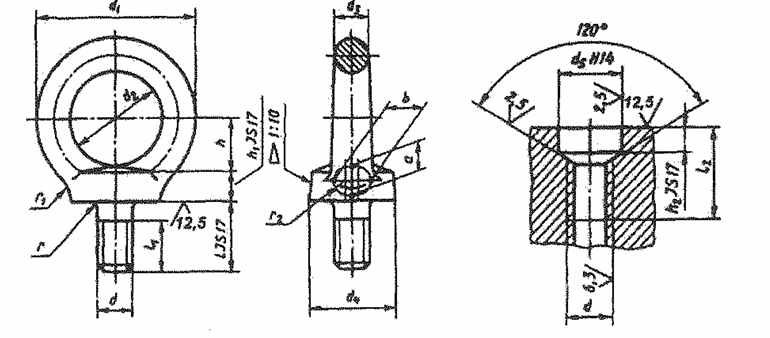
\includegraphics[width=0.8\textwidth]{pictures/ring_screw.png}
                \caption{Vít vòng}
                \label{ring_screw}
            \end{figure}
            \hspace*{0.6cm}Để nâng và vận chuyển hộp giảm tốc trên nắp và thân thường ngoài bu lông ta sử dụng vòng móc. \\
            \hspace*{0.6cm}Do đây hộp giảm tốc bánh răng trụ 1 cấp và khoảng cách trục $a = 160$ mm. Từ bảng 10.7, tài liệu tham khảo \cite{tkmctm} $\rightarrow$ Trọng lượng hộp giảm tốc $Q = 80$ (kg). \\
            \hspace*{0.6cm}Từ bảng 10.6, tài liệu tham khảo \cite{tkmctm}, ta chọn vít vòng M8 với các thông số: 
            \begin{longtable}{|c|c|}
                \hline
                \textbf{Thông số} & \textbf{Giá trị (mm)} \\
                \hline
                Đường kính vít vòng $d$ & 8 \\
                \hline
                Đường kính vòng ngoài, $d_1$ & 36 \\
                \hline
                Đường kính vòng trong, $d_2$ & 20 \\
                \hline
                $d_3$ & 8 \\  
                \hline
                $d_4$ & 20 \\
                \hline
                $b$ & 10 \\
                \hline
                $h$ & 12 \\
                \hline
                $h_1$ & 6 \\
                \hline
                $l$ & 18 \\
                \hline
                $l_1$, lớn hơn & 12 \\
                \hline
                $r$ & 2 \\
                \hline
                $r_1$ & 4 \\
                \hline
                Khối lượng & 0.05 \\
                \hline
                \centering $d_5$ & 13 \\
                \hline
                $h_2$ & 5 \\
                \hline
                \centering $l_2$, lớn hơn & 19 \\
                \hline
                \caption{Thông số vít vòng}
            \end{longtable}
        \subsection{Chốt định vị}
            \hspace*{0.6cm}Đảm bảo vị trí tương đối giữa nắp và thân hộp trước và sau khi gia công cũng như khi lắp ghé, dùng 2 chốt định vị. Nhờ chốt định vị, khi siết bulông không làm biến dạng vòng ngoài của ổ (do sai lệch vị trí tương đối của nắp và thân hộp), do đó làm loại trừ một trong các nguyên nhân làm ổ chóng hỏng.\\
            \hspace*{0.6cm}Chọn chốt hình côn, có thông số như sau:
            \begin{figure}[H]
                \centering
                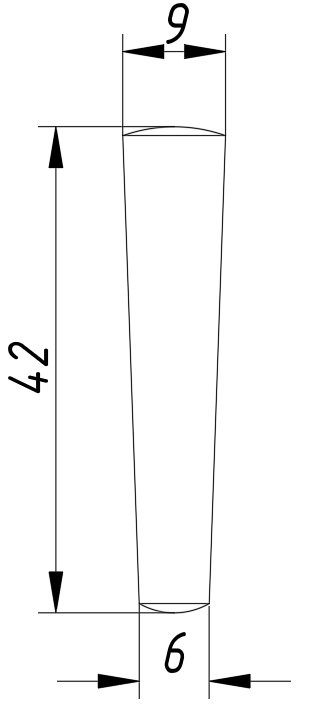
\includegraphics[width=0.2\textwidth]{pictures/position_pin.png}
                \caption{Chốt định vị}
                \label{position_pin}
            \end{figure}
            \begin{table}[H]
                \centering
                \begin{tabular}{|c|c|c|c|}
                    \hline
                    \textbf{Thông số} & $\mathbf{d_1}$ & $\mathbf{d}$ & $\mathbf{l}$ \\
                    \hline
                    \textbf{Giá trị (mm)} & 9 & 42 & 6 \\
                    \hline
                \end{tabular}     
                \caption{Thông số chốt định vị}           
            \end{table}
        \subsection{Cửa thăm}
            \begin{figure}[H]
                \centering
                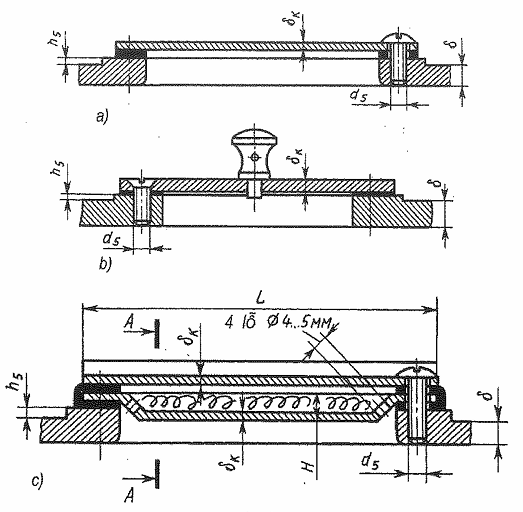
\includegraphics[width=0.6\textwidth]{pictures/oil_dipstick_cap.png}
                \caption{Nắp cửa thăm}
                \label{oil_dipstick_cap}
            \end{figure}
            \hspace*{0.6cm}Để kiểm tra, quan sát các chi tiết máy trong hộp khi lắp ghép và để đổ dầu vào hộp, trên đỉnh hộp có làm cửa thăm. Cửa thăm được đậy bằng nắp. Trên nắp có lắp thêm nút thông hơi \\
            \hspace*{0.6cm}Kích thước nắp cửa thăm dầu:
            \begin{longtable}{|c|c|c|c|c|c|c|c|c|c|}
                \hline
                \textbf{Thông số} & $\mathbf{A}$ & $\mathbf{B}$ & $\mathbf{A_1}$ & $\mathbf{B_1}$ & $\mathbf{C}$ & $\mathbf{K}$ & $\mathbf{R}$ & \textbf{Kích thước vít} & \textbf{Số vít}\\
                \hline
                \textbf{Giá trị (mm)} & 100 & 75 & 150 & 12O & 125 & 100 & 12 & M8x22 & 4 \\
                \hline
                \caption{Thông số nắp cửa thăm}
            \end{longtable}
        \subsection{Nút thông hơi}
            \hspace*{0.6cm}Khi làm việc, nhiệt độ trong hộp tăng lên. Để giảm áp suất và điều hòa không khí bên trong và ngoài hộp. Ta dùng nút thông hơi. Nút thông hơi được lắp trên nắp cửa thăm.
            \begin{figure}[H]
                \centering
                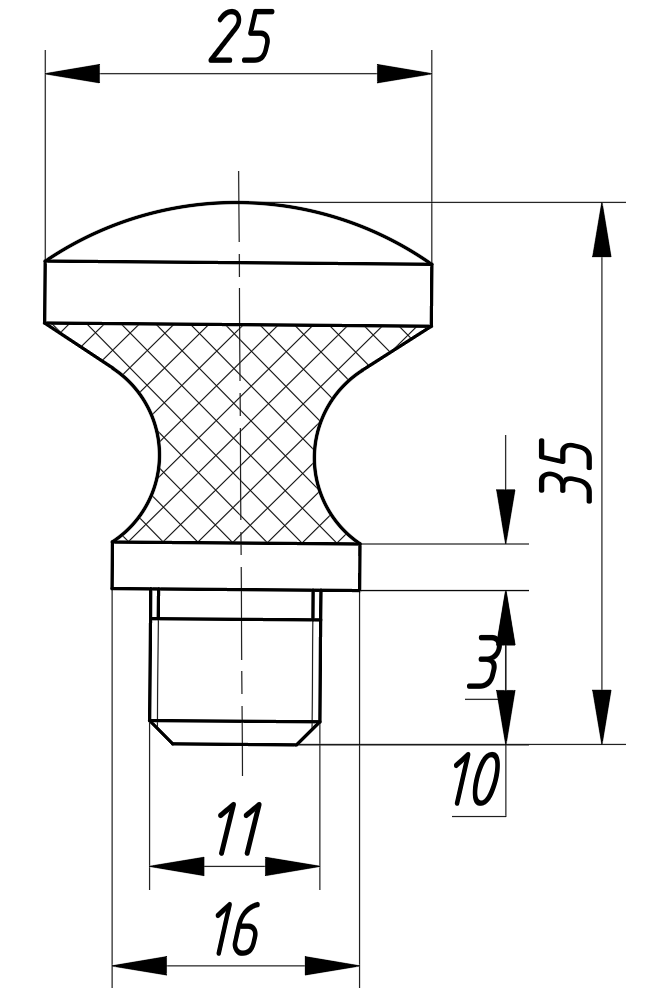
\includegraphics[width=0.3\textwidth]{pictures/ven_plug.png}
                \caption{Nút thông hơi}
                \label{ven_plug}
            \end{figure} 
            \begin{table}[H]
                \centering
                \begin{tabular}{|c|c|c|c|c|c|c|}
                    \hline
                    \textbf{Thông số} & $\mathbf{d}$ & $\mathbf{D}$ & $\mathbf{D_1}$ & $\mathbf{L}$ & $\mathbf{l}$ & $\mathbf{b}$  \\
                    \hline
                    \textbf{Giá trị (mm)} & M11x1.75 & 16 & 25 & 35 & 10 & 3 \\
                    \hline 
                \end{tabular}     
                \caption{Thông số nút thông hơi}           
            \end{table}
        \subsection{Nút tháo dầu}
            \hspace*{0.6cm}Sau một thời gian làm việc, dầu bôi trơn chứa trong hộp bị bẩn (do bụi bặm và do hạt mài) hoặc bị biến chất, do đó cần phải thay dầu mới. Để tháo dầu, ở đáy hộp có lỗ tháo dầu. Khi làm việc, lỗ được bít kín bằng nút tháo dầu. Thông số nút tháo dầu được tham khảo bảng 18-7 tài liệu tham khảo \cite{tltk2}.\\ 
            \begin{figure}[H]
                \centering
                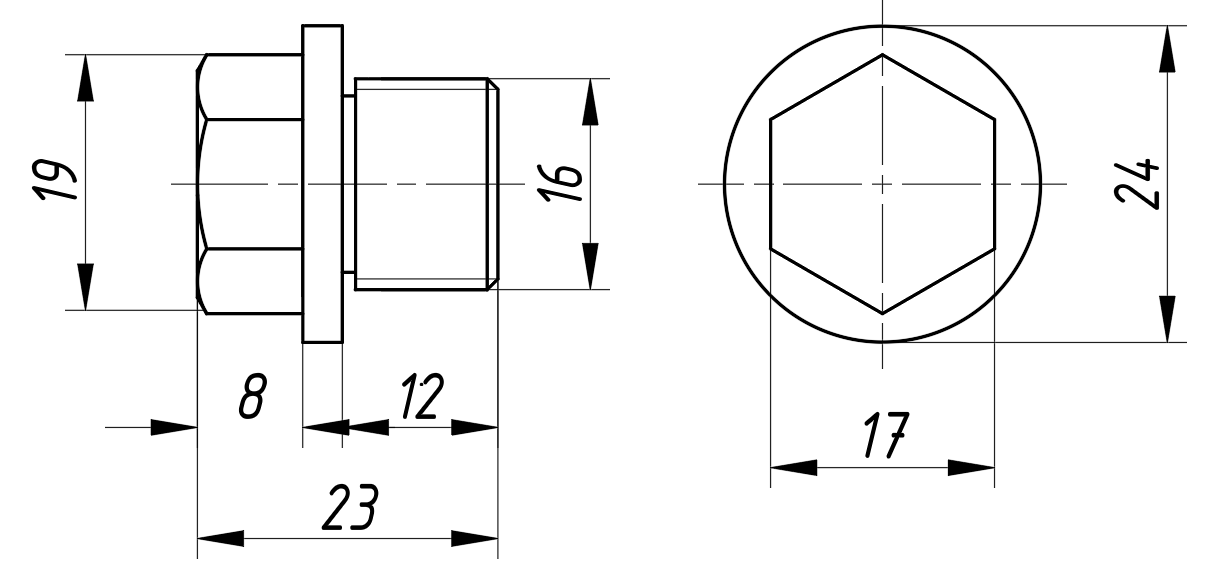
\includegraphics[width=0.7\textwidth]{pictures/oil_drain_plug.png}
                \caption{Nút tháo dầu}
                \label{oil_drain_plug}
            \end{figure}
            \begin{table}[H]
                \centering
                \begin{tabular}{|c|c|}
                    \hline
                    \textbf{Thông số} & \textbf{Giá trị (mm)} \\
                    \hline
                    $\mathbf{d}$ & M16x1.5 \\     
                    \hline
                    $\mathbf{b}$ & 12 \\
                    \hline
                    $\mathbf{m}$ & 8 \\
                    \hline
                    $\mathbf{f}$ & 3 \\
                    \hline
                    $\mathbf{L}$ & 23 \\
                    \hline
                    $\mathbf{c}$ & 2 \\
                    \hline
                    $\mathbf{q}$ & 13.8 \\
                    \hline
                    $\mathbf{D}$ & 26 \\
                    \hline
                    $\mathbf{S}$ & 17 \\
                    \hline
                    $\mathbf{D_{0}}$ & 19.6 \\
                    \hline
                \end{tabular}     
                \caption{Thông số nút tháo dầu}
            \end{table}
        \subsection{Que thăm dầu}
            \hspace*{0.6cm}Để kiểm tra mức dầu trong hộp, ta dùng que thăm dầu.\\
            \hspace*{0.6cm}Que thăm dầu có các thông số như sau:
            \begin{figure}[H]
                \centering
                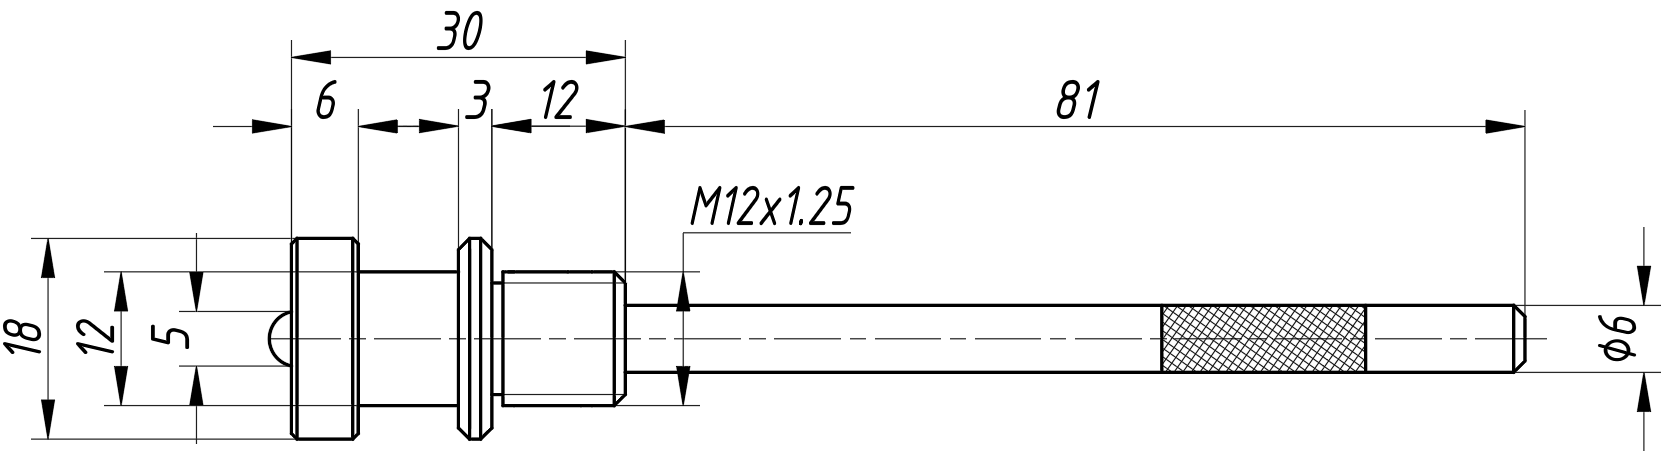
\includegraphics[width=0.7\textwidth]{pictures/oil_dipstick.png}
                \caption{Que thăm dầu}
                \label{oil_dipstick}
            \end{figure}
            \begin{table}[H]
                \centering
                \begin{tabular}{|c|c|c|c|c|c|c|c|c|c|}
                    \hline
                    \textbf{Thông số} & $\mathbf{d}$ & $\mathbf{d_1}$ & $\mathbf{d_2}$ & $\mathbf{D}$ & $\mathbf{D_1}$ & $\mathbf{L_1}$ & $\mathbf{l}$ & $\mathbf{l_1}$ & $\mathbf{b}$ \\
                    \hline
                    \textbf{Giá trị (mm)} & M12x1.25 & 5 & 6 & 18 & 12 & 30 & 12 & 6 & 3 \\
                    \hline
                \end{tabular}     
                \caption{Thông số que thăm dầu}           
            \end{table}
        \subsection{Vòng phớt}
            \hspace*{0.6cm}Vòng phớt là loại lót kín động gián tiếp nhằm mục đích bảo vệ ổ khỏi bụi bặm, chất bẩn, hạt cứng và các tạp chất khác xâm nhập vào ổ. Những chất này làm ổ chóng bị mài mòn và bị han gỉ. Ngoài ra, vòng phớt còn đề phòng dầu chảy ra ngoài. Tuổi thọ ổ lăn phụ thuộc rất nhiều vào vòng phớt. \\
            \hspace*{0.6cm}Vòng phớt được dùng khá rộng rãi do có kết cấu đơn giản, thay thế dễ dàng. Tuy nhiên có nhược điểm là chóng mòn và ma sát lớn khi bề mặt trục có độ nhám cao. 
            \begin{figure}[H]
                \centering
                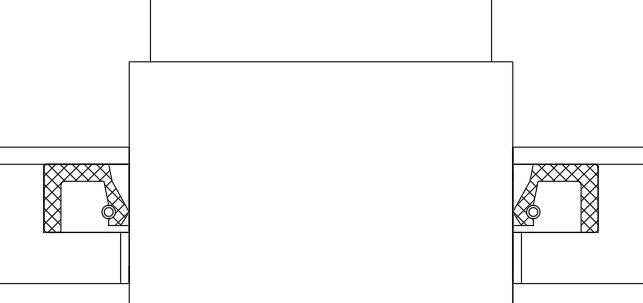
\includegraphics[width=0.5\textwidth]{pictures/seal.png}
                \caption{Vòng phớt}
                \label{seal}
            \end{figure}
        \subsection{Vòng chắn dầu}
            \hspace*{0.6cm}Vòng chắn dầu dùng để ngăn mỡ trong ổ và dầu trong hộp. Vòng gồm 3 rãnh tiết diện tam giác có góc ở đỉnh 60$^\circ$. Khoảng cách giữa các đỉnh là 3 (mm). Vòng cách mép trong thành hộp khoảng (0.5 $\div$ 1) (mm). Khe hở giữa vỏ với mặt ngoài của vòng ren là 0.43 (mm).
            \begin{figure}[H]
                \centering
                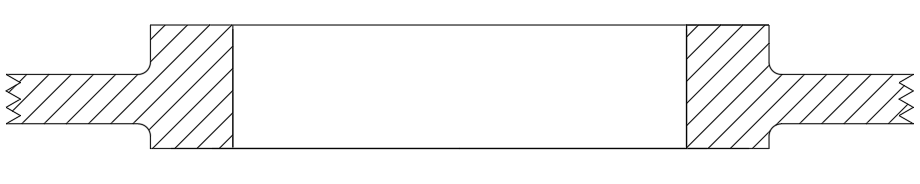
\includegraphics[width=0.5\textwidth]{pictures/oil_shield.png}
                \caption{Vòng chắn dầu}
                \label{oil_shield}
            \end{figure}
           
            
        \chapter{BÔI TRƠN, DUNG SAI VÀ LẮP GHÉP}
    \section{BÔI TRƠN}
        \subsection{Bôi trơn trong hộp giảm tốc}
            \begin{itemize}
                \item Do các bộ truyền bánh răng trong hộp giảm tốc đều có $v > 12 m/s$ nên ta chọn phương pháp bôi trơn ngâm dầu. Lượng dầu bôi trơn thường vào khoảng $0.4 \div 0.8$ lít cho 1kW công suất truyền. Với vận tốc của bánh cấp nhanh $v = 5.03 m/s$, vật liệu thép C45, tra bảng 18-11 tài liệu tham khảo \cite{tltk2} ta được độ nhớt 80/11 ứng với 500C. 
                \item Theo bảng 18-13 tài liệu tham khảo \cite{tltk2}, ta chọn loại dầu bôi trơn là dầu Ôt máy kéo AK20. 
            \end{itemize}
        \subsection{Lắp bánh răng lên trục và điều chỉnh sự ăn khớp}
            \begin{itemize}
                \item Đối với bánh răng côn, việc điều chỉnh được tiến hành trên cả hai bánh răng dẫn và bị dẫn.
                \item Dịch chuyển trục cùng với các bánh răng đã cố định trên nó nhờ bộ đệm điều chỉnh có chiều dày khác nhau lắp giữa nắp ổ và vỏ hộp. Việc điều chỉnh như thế này khá thuận tiện. Dịch chuyển các bánh răng trên trục đã cố định, sau đó định vị lần lượt từng bánh một. Việc điều chỉnh này khá phức tạp.
                \item Lưu ý: Độ điều chỉnh phải đạt tối thiểu là $70\%$ trên bề mặt răng.
            \end{itemize}
    \section{CHỌN CẤP CHÍNH XÁC}
        \begin{itemize}
            \item Đối với hệ thống trục, chọn cấp chính xác là 6. Vì gia công lỗ phức tạp hơn gia công trục, do đó chọn cấp chính xác gia công lỗ thấp hơn trục 1 cấp, ta chọn cấp 7.
            \item Đối với bánh răng, chọn cấp chính xác là 9 như đã tính toán.
        \end{itemize}
    \section{CHỌN KIỂU LẮP}
        \subsection{Bánh răng bị dẫn}
            \hspace*{0.6cm}Chọn kiểu lắp H7/k6 do mối ghép không yêu cầu tháo lắp thường xuyên, bánh răng lắp trên trục chịu tải trọng tĩnh, vừa, va đập nhẹ.
        \subsection{Ổ lăn}
            \hspace*{0.6cm}Vòng trong ổ lăn chịu tải tuần hoàn, ta lắp ghép theo hệ thống trục lắp trung gian để vòng ổ không trượt trên bề mặt trục khi làm việc. Do đó, ta phải chọn mối lắp k6, lắp trung gian có độ dôi, tạo điều kiện mòn đều ổ (trong quá trình làm việc nó sẽ quay làm mòn đều). \\
            \hspace*{0.6cm}Vòng ngoài của ổ lăn không quay nên chịu tải cục bộ, ta lắp theo hệ thống lỗ. Để ổ có thể di chuển dọc trục khi nhiệt đô tăng trong quá trình làm việc, ta chọn kiểu lắp trung gian H7.
        \subsection{Then}
            \hspace*{0.6cm}Trong mối ghép then, kích thước lắp ghép là bề rộng b của then. Đối với trục, ta chọn kiểu lắp trung gian N9/H9, đối với bạc ta chọn kiểu lắp trung gian Js9/h9.
        \subsection{Vòng chắn dầu}
            \hspace*{0.6cm}Vì vòng chắn dầu cần quay theo trục để dầu bên ngoài không bắn vào trong ổ lăn và dễ dang tháo lắp nên ta chọn lắp trung gian H7/js6.
        \subsection{Vòng phớt và nắp ổ}
            \hspace*{0.6cm}Để mối ghép cố định khi làm việc nhưng các chi tiết dễ dàng dịch chuyển với nhau khi điều chỉnh nên ta chọn kiểu lắp hở H7/h6 cho nắp ổ lăn và H8/e8 cho vòng phớt. 
    \section{BẢNG DUNG SAI}
        \subsection{Bảng dung sai lắp ghép bánh răng}
            \begin{table}[H]
                \centering
                \begin{tabular}{|c|c|c|c|c|c|c|}
                    \hline
                    \textbf{Mối lắp} & \textbf{Kích thước} & \textbf{Kiểu lắp} & $\mathbf{es (\mu m)}$ & $\mathbf{ei (\mu m)}$ & $\mathbf{ES (\mu m)}$ & $\mathbf{EI (\mu m)}$\\
                    \hline
                    Bánh đai & $\phi 22$ & H7/k6 & 15 & 2 & 21 & 0 \\
                    \hline
                    Bánh răng bị dẫn & $\phi 60$ & H7/k6 & 21 & 2 & 30 & 0 \\
                    \hline
                    Bánh răng côn dẫn & $\phi 40$ & H7/k6 & 18 & 2 & 25 & 0 \\
                    \hline
                \end{tabular}
                \caption{Bảng dung sai lắp ghép bánh răng}
            \end{table}
        \subsection{Bảng dung sai lắp ghép then}
            \begin{table}[H]
                \centering
                \begin{tabular}{|c|c|c|c|c|}
                    \hline
                    \multirow{3}{*}{\begin{tabular}[c]{@{}c@{}}Kích thước tiết\\diện then\\$b \times h$\end{tabular}} &
                    \multicolumn{2}{c|}{\begin{tabular}[c]{@{}c@{}}Sai lệch giới hạn\\chiều rộng rãnh then\end{tabular}} &
                    \multicolumn{2}{c|}{Chiều sâu rãnh then} \\
                    \cline{2-5}
                    &\begin{tabular}[c]{@{}c@{}}Trên\\trục\end{tabular} &
                    \begin{tabular}[c]{@{}c@{}}Trên\\bạc\end{tabular} &
                    \multirow{2}{*}{\begin{tabular}[c]{@{}c@{}}Sai lệch giới hạn\\trên trục $t_1$\end{tabular}} &
                    \multirow{2}{*}{\begin{tabular}[c]{@{}c@{}}Sai lệch giới hạn\\trên bạc $t_2$\end{tabular}} \\
                    \cline{2-3}
                    & N9 & Js9 & & \\
                    \hline
                    $6 \times 6$ &
                    \begin{tabular}[c]{@{}c@{}}0\\-0.036\end{tabular} &
                    \begin{tabular}[c]{@{}c@{ }}+0.018\\-0.018\end{tabular} &
                    0.2 & 0.2 \\
                    \hline
                    $18 \times 11$ &
                    \begin{tabular}[c]{@{}c@{}}0\\-0.043\end{tabular} &
                    \begin{tabular}[c]{@{}c@{}}+0.0215\\-0.0215\end{tabular} &
                    0.2 & 0.2 \\
                    \hline
                    $12 \times 8$ &
                    \begin{tabular}[c]{@{}c@{}}0\\-0.043\end{tabular} &
                    \begin{tabular}[c]{@{}c@{}}+0.0215\\-0.0215\end{tabular} &
                    0.2 & 0.2 \\
                    \hline
                \end{tabular}
                \caption{Bảng dung sai lắp ghép then}
            \end{table}
    \subsection{Bảng dung sai lắp ghép ổ lăn}
        \begin{table}[H]
            \centering
            \begin{tabular}{|c|c|c|c|c|c|}
                \hline
                Mối lắp & Kiểu lắp & es ($\mu m$) & ei ($\mu m$) & ES ($\mu m$) & EI ($\mu m$) \\
                \hline
                Vòng trong ổ trục II & $\varnothing30k6$ & +18 & +2 & & \\
                \hline
                Vòng trong ổ trục III & $\varnothing50k6$ & +18 & +2 & & \\
                \hline
                Vòng ngoài ổ trục II & $\varnothing62H7$ & & & +30 & 0 \\
                \hline
                Vòng ngoài ổ trục III & $\varnothing110H7$ & & & +35 & 0 \\
                \hline
            \end{tabular}
            \caption{Bảng dung sai lắp ghép ổ lăn}
        \end{table}
    \subsection{Bảng dung sai các chi tiết khác}
        \begin{table}[htbp]
            \centering
            \begin{tabular}{|c|c|c|c|c|c|c|}
                \hline
                Mối lắp & Kích thước & Kiểu lắp & es ($\mu m$) & ei ($\mu m$) & ES ($\mu m$) & EI ($\mu m$) \\
                \hline
                Nắp ổ trục II & $\varnothing62$ & H7/h6 & 0 & -19 & +30 & 0 \\
                \hline
                Nắp ổ trục III & $\varnothing110$ & H7/h6 & 0 & -22 & +35 & 0 \\
                \hline
                Vòng chặn đầu trục II & $\varnothing35$ & H7/js6 & +8 & -8 & +25 & 0 \\
                \hline
                Vòng chặn đầu trục III & $\varnothing55$ & H7/js6 & +9,5 & -9,5 & +30 & 0 \\
                \hline
                Vòng phớt trục II & $\varnothing25$ & H8/e8 & -40 & -73 & +33 & 0 \\
                \hline
                Vòng phớt trục III & $\varnothing45$ & H8/e8 & -50 & -89 & +39 & 0 \\
                \hline
            \end{tabular}
            \caption{Bảng dung sai các chi tiết khác}
        \end{table}

            
            
        \nocite{*}
        \printbibliography[title={TÀI LIỆU THAM KHẢO}, heading=bibintoc]
\end{document}